\documentclass[a4paper,11pt]{article}

% ============================================================
%  Le Collé — Séries entières
%  © 2026 Ahmed Amine Ouqlani
% ============================================================

% ---------- Polices ----------
\usepackage[utf8]{inputenc}
\usepackage[T1]{fontenc}
\usepackage[sc]{mathpazo}          % texte et mathématiques : Palatino
\usepackage[scaled=0.88]{helvet}   % titres et repères : linéale
\linespread{1.07}
\usepackage{amsmath,amssymb,amsthm,mathrsfs,stmaryrd}
\usepackage{microtype}

% ---------- Mise en page ----------
\usepackage[a4paper,top=2.3cm,bottom=2.3cm,left=2.4cm,right=2.4cm,
            headheight=14pt,headsep=0.8cm,footskip=1.1cm]{geometry}
\setlength{\parindent}{0pt}
\setlength{\parskip}{0.45em plus 0.15em minus 0.1em}
\raggedbottom
\emergencystretch=1.5em
\clubpenalty=10000 \widowpenalty=10000 \displaywidowpenalty=10000 \brokenpenalty=10000

% ---------- Couleurs : un bleu de nuit, un ocre, des gris ----------
\usepackage{xcolor}
\definecolor{Ink}{HTML}{1C2533}
\definecolor{Bleu}{HTML}{1F3A5F}
\definecolor{BleuMoyen}{HTML}{4A6A8F}
\definecolor{BleuClair}{HTML}{9DB2C9}
\definecolor{Fond}{HTML}{F2F4F7}
\definecolor{Ocre}{HTML}{B07A26}
\definecolor{Brique}{HTML}{A23B2A}
\definecolor{Gris}{HTML}{5E6672}
\definecolor{Filet}{HTML}{C5CCD6}

% ---------- Packages ----------
\usepackage{enumitem}
\setlist{itemsep=0.25em,topsep=0.35em,parsep=0pt}
\setlist[itemize]{label=\textcolor{BleuMoyen}{\small\textbullet},leftmargin=1.4em}
\setlist[enumerate]{leftmargin=1.8em,label=\textsf{\small\color{Bleu}\arabic*.}}
\usepackage{booktabs,array,multicol}
\usepackage{needspace,float}
\usepackage[font=small,labelfont={sf,color=Bleu},labelsep=period,skip=6pt]{caption}
\usepackage{tikz}
\usetikzlibrary{arrows.meta,calc,decorations.markings}
\usepackage{pgfplots}
\pgfplotsset{compat=1.17}
\usepackage{tkz-tab}
\usepackage[most]{tcolorbox}
\usepackage{titlesec,titletoc}
\usepackage{fancyhdr,lastpage,etoolbox}
\usepackage[colorlinks=true,linkcolor=Bleu,urlcolor=Bleu,citecolor=Bleu,
            pdftitle={Le Collé — Séries entières},pdfauthor={Ahmed Amine Ouqlani}]{hyperref}

\numberwithin{equation}{section}
\numberwithin{figure}{section}
\numberwithin{table}{section}

% ---------- Titres ----------
% numéro du chapitre dans le parcours PT (affiché), distinct de la numérotation interne
\newcommand{\grandnum}{\thesection}\newcommand{\ongletcouleur}{Bleu}
% Chapitres (sections) : grand numéro, titre en linéale, filet ocre
\titleformat{\section}[display]
  {\normalfont\sffamily\color{Ink}}
  {{\small\color{Gris}\textls[200]{\MakeUppercase{Chapitre}}}\\[-0.2em]%
   {\fontsize{64}{64}\selectfont\color{BleuClair}\grandnum}}
  {0.4em}
  {\fontsize{25}{30}\selectfont\bfseries}
  [\vspace{0.5em}{\color{Ocre}\rule{3.2cm}{1.4pt}}]
\titlespacing*{\section}{0pt}{0pt}{1.6em}
\titleformat{name=\section,numberless}[display]
  {\normalfont\sffamily\color{Ink}}{}{0pt}{\fontsize{25}{30}\selectfont\bfseries}
  [\vspace{0.5em}{\color{Ocre}\rule{3.2cm}{1.4pt}}]
\titlespacing*{name=\section,numberless}{0pt}{0pt}{1.6em}

\titleformat{\subsection}
  {\needspace{5\baselineskip}\normalfont\sffamily\Large\bfseries\color{Ink}}
  {\color{Bleu}\thesubsection}{0.8em}{}
\titlespacing*{\subsection}{0pt}{1.8em}{0.5em}
\titleformat{\subsubsection}
  {\needspace{5\baselineskip}\normalfont\sffamily\large\bfseries\color{Ink}}
  {\color{Bleu}\thesubsubsection}{0.7em}{}
\titlespacing*{\subsubsection}{0pt}{1.6em}{0.4em}
\titleformat{\paragraph}[runin]{\normalfont\sffamily\bfseries\color{Ink}}{}{0pt}{}[.]
\titlespacing*{\paragraph}{0pt}{0.9em}{0.6em}
\setcounter{secnumdepth}{3}
\setcounter{tocdepth}{2}

% ---------- Table des matières ----------
\titlecontents{section}[0pt]{\addvspace{0.7em}\sffamily\bfseries\color{Ink}}
  {}{}{\hfill\contentspage}[\addvspace{0.2em}]
\titlecontents{subsection}[2.2em]{\small\linespread{1}\selectfont}
  {\makebox[2.6em][l]{\color{Gris}\thecontentslabel}}{}{\titlerule*[0.7pc]{.}\contentspage}

% ---------- En-têtes et pieds de page ----------
\pagestyle{fancy}
\fancyhf{}
\renewcommand{\sectionmark}[1]{\markboth{#1}{}}
\fancyhead[L]{\footnotesize\sffamily\color{Gris}\leftmark}
\fancyhead[R]{\footnotesize\sffamily\scshape\color{Gris}Le Collé}
\fancyfoot[C]{\small\sffamily\color{Ink}\thepage}
\fancyfoot[L]{\scriptsize\sffamily\hyperlink{toc}{\color{Filet}sommaire}}
\renewcommand{\headrulewidth}{0.4pt}
\renewcommand{\headrule}{{\color{Filet}\hrule height\headrulewidth width\headwidth}}
\renewcommand{\footrulewidth}{0pt}
\fancypagestyle{plain}{\fancyhf{}\fancyfoot[C]{\small\sffamily\color{Ink}\thepage}\renewcommand{\headrulewidth}{0pt}}

% ---------- Énoncés ----------
\newtheoremstyle{enonce}{0pt}{0pt}{}{}{\sffamily\bfseries\color{Bleu}}{.}{0.5em}
  {\thmname{#1}\thmnumber{~#2}\thmnote{\ \normalfont\sffamily\color{Ink}(#3)}}
\newtheoremstyle{exemple}{0.9em}{0.9em}{}{}{\sffamily\bfseries\color{BleuMoyen}}{.}{0.5em}
  {\thmname{#1}\thmnumber{~#2}\thmnote{\ \normalfont\sffamily\color{Ink}(#3)}}
\newtheoremstyle{remarque}{0.7em}{0.7em}{}{}{\sffamily\itshape}{.}{0.5em}{\thmname{#1}\thmnote{\ (#3)}}
\theoremstyle{enonce}
\newtheorem{definition}{Définition}[section]
\newtheorem{theoreme}[definition]{Théorème}
\newtheorem{proposition}[definition]{Proposition}
\newtheorem{corollaire}[definition]{Corollaire}
\theoremstyle{exemple}
\newtheorem{exemple}[definition]{Exemple}
\theoremstyle{remarque}
\newtheorem*{remarque}{Remarque}

\tcbset{
  defi/.style={enhanced,breakable,colback=white,colframe=white,boxrule=0pt,arc=0pt,
     borderline west={1.2pt}{0pt}{Bleu},left=11pt,right=4pt,top=3pt,bottom=3pt,
     before skip=1.1em,after skip=1.1em},
  thm/.style={enhanced,breakable,colback=Fond,colframe=Fond,boxrule=0pt,arc=0pt,
     borderline west={2.4pt}{0pt}{Bleu},left=11pt,right=8pt,top=6pt,bottom=6pt,
     before skip=1.2em,after skip=1.2em}}
\tcolorboxenvironment{definition}{defi}
\tcolorboxenvironment{theoreme}{thm}
\tcolorboxenvironment{proposition}{thm}
\tcolorboxenvironment{corollaire}{thm}

\renewcommand{\proofname}{Démonstration}
\renewcommand{\qedsymbol}{\textcolor{BleuClair}{$\blacksquare$}}
\makeatletter
\renewenvironment{proof}[1][\proofname]{\par\pushQED{\qed}\normalfont
  \topsep0.5em\relax\trivlist\item[\hskip\labelsep\sffamily\itshape\color{Gris}#1.]\ignorespaces}
  {\popQED\endtrivlist\@endpefalse}
\makeatother

% ---------- Méthode : filets haut et bas, titre en bandeau ----------
\makeatletter\newcommand{\methlabelfix}{\protected@edef\@currentlabel{\thetcbcounter}}\makeatother
\newtcolorbox[auto counter,number within=section]{methode}[2][]{%
  enhanced,unbreakable,colback=white,colframe=white,boxrule=0pt,arc=0pt,
  borderline north={0.9pt}{0pt}{Bleu},borderline south={0.9pt}{0pt}{Bleu},
  left=4pt,right=4pt,top=8pt,bottom=8pt,before skip=1.4em,after skip=1.4em,
  before upper={\methlabelfix\phantomsection\addcontentsline{met}{metentry}{\protect\makebox[2.6em][l]{\thetcbcounter}#2}%
     {\sffamily\bfseries\small\color{white}\colorbox{Bleu}{\strut\ MÉTHODE~\thetcbcounter\ }}%
     \ \ {\sffamily\bfseries\color{Bleu}#2}\par\smallskip},#1}

% ---------- Repères pédagogiques : un filet de couleur, un mot-clé ----------
\newcommand{\definirbloc}[3]{% nom, couleur, libellé
  \newtcolorbox{#1}[1][]{enhanced,breakable,blanker,
    borderline west={1.4pt}{0pt}{#2},left=10pt,right=2pt,top=1pt,bottom=1pt,
    before skip=1em,after skip=1em,
    before upper={{\sffamily\bfseries\footnotesize\color{#2}\textls[120]{\MakeUppercase{#3}}}\quad},##1}}
\definirbloc{reflexe}{Bleu}{Réflexe}
\definirbloc{astuce}{Ocre}{Astuce}
\definirbloc{attention}{Brique}{Attention}
\definirbloc{enpratique}{BleuMoyen}{En pratique}
\definirbloc{plusloin}{Gris}{Pour aller plus loin}
\definirbloc{strategie}{Bleu}{Stratégie}
\definirbloc{lecture}{BleuMoyen}{Lire le schéma}
% compatibilité avec les parties reprises
\newenvironment{garde}{\begin{attention}}{\end{attention}}
\newenvironment{complementHP}{\begin{plusloin}}{\end{plusloin}}
\newenvironment{interpretation}{\begin{enpratique}}{\end{enpratique}}

% ---------- Exercices, corrigés ----------
\newcounter{exo}[section]
\renewcommand{\theexo}{\thesection.\arabic{exo}}
\newcommand{\niveau}[1]{{\color{Ocre}\footnotesize
  \ifcase#1\or$\bullet\circ\circ\circ\circ$\or$\bullet\bullet\circ\circ\circ$\or$\bullet\bullet\bullet\circ\circ$%
  \or$\bullet\bullet\bullet\bullet\circ$\or$\bullet\bullet\bullet\bullet\bullet$\fi}}
\newcommand{\serie}[1]{\par\needspace{8\baselineskip}\vspace{1.5em}%
  \noindent{\sffamily\bfseries\color{Bleu}#1}\par\nobreak\vspace{-0.4em}%
  \noindent{\color{Filet}\rule{\linewidth}{0.4pt}}\par\nobreak\vspace{0.1em}}
\newenvironment{exo}[3]{%
  \par\needspace{5\baselineskip}\vspace{0.75em}\refstepcounter{exo}\label{e:#1}%
  \def\exolab{#1}%
  \noindent{\sffamily\bfseries\color{Bleu}Exercice~\theexo}\quad\niveau{#2}%
  \hfill{\footnotesize\sffamily\color{Gris}#3}\par\nobreak\vspace{0.15em}}%
  {\par\nopagebreak\noindent\hfill{\scriptsize\sffamily\hyperref[c:\exolab]{\color{Gris}corrigé p.~\pageref{c:\exolab}}}\par}
\newenvironment{corrige}[1]{%
  \par\needspace{6\baselineskip}\vspace{1em}\phantomsection\label{c:#1}%
  \noindent{\sffamily\bfseries\color{Bleu}Exercice~\ref{e:#1}}\quad
  {\scriptsize\sffamily\hyperref[e:#1]{\color{Gris}énoncé p.~\pageref{e:#1}}}\par\nobreak\vspace{0.2em}}%
  {\hfill\textcolor{BleuClair}{$\square$}\par}
\newcommand{\etape}[1]{\par\smallskip\noindent{\sffamily\bfseries\small\color{BleuMoyen}#1.}\ }
\newenvironment{solution}{\par\noindent{\sffamily\bfseries\small\color{BleuMoyen}Solution.}\ }{\hfill\textcolor{BleuClair}{$\square$}\par}
\newcommand{\chercher}{\par\smallskip\noindent{\color{Filet}\rule[0.5ex]{1.2cm}{0.4pt}}\
  {\footnotesize\sffamily\itshape\color{Gris}laisser chercher l'étudiant avant de poursuivre}\par\smallskip}

% ---------- Guide de séance ----------

\newcommand{\marge}[1]{\leavevmode\marginpar{\raggedleft\scriptsize\sffamily\color{Gris}\textls[100]{\MakeUppercase{#1}}}\ignorespaces}
\newcommand{\Etape}[4]{%
  \subsection[Étape #1 --- #3 {\color{Gris}(#2)}]{#3}\label{etape:#1}%
  \noindent{\small\sffamily\color{Gris}{\color{Ocre}\bfseries Étape #1}\quad·\quad #2\quad·\quad #4}\par\medskip}
\newcommand{\question}[1]{\par\smallskip\noindent{\sffamily\bfseries\small\color{BleuMoyen}Question.}\ \textit{#1}\par\smallskip}
\newcommand{\rappel}[1]{\par\smallskip\noindent\phantomsection\addcontentsline{rap}{rapentry}{#1}%
  {\sffamily\bfseries\scriptsize\colorbox{Fond}{\color{Gris}\strut RAPPEL}}\ {\sffamily\small\color{Gris}#1.}\ }
\newcommand{\pourquoi}{\par\noindent{\sffamily\bfseries\small\color{Ocre}Pourquoi ?}\ }

% Ouverture de chapitre : \ouverture{objectifs}{prérequis}{durée}
\newcommand{\ouverture}[3]{%
  \begin{tcolorbox}[enhanced,colback=Fond,colframe=Fond,arc=0pt,boxrule=0pt,left=12pt,right=12pt,top=10pt,bottom=10pt,
     before skip=1.2em,after skip=1.6em]
  \begin{minipage}[t]{0.56\linewidth}
  {\sffamily\bfseries\small\color{Bleu}OBJECTIFS}\par\vspace{0.3em}\small #1
  \end{minipage}\hfill
  \begin{minipage}[t]{0.38\linewidth}
  {\sffamily\bfseries\small\color{Bleu}PRÉREQUIS}\par\vspace{0.3em}\small #2
  \ifx\relax#3\relax\else\par\vspace{0.6em}{\sffamily\bfseries\small\color{Bleu}DURÉE}\par\vspace{0.2em}\small #3\fi
  \end{minipage}
  \end{tcolorbox}}
% Fin de chapitre
\newenvironment{essentiel}{\par\needspace{12\baselineskip}\vspace{1.5em}%
  \begin{tcolorbox}[enhanced,unbreakable,colback=white,colframe=white,boxrule=0pt,arc=0pt,
   borderline north={1.4pt}{0pt}{Ocre},left=2pt,right=2pt,top=8pt,bottom=4pt]
  {\sffamily\bfseries\color{Ocre}L'ESSENTIEL DU CHAPITRE}\par\medskip}{\end{tcolorbox}}

% ---------- Notations ----------
\newcommand{\K}{\mathbb{K}}
\newcommand{\R}{\mathbb{R}}
\newcommand{\C}{\mathbb{C}}
\newcommand{\N}{\mathbb{N}}
\newcommand{\Z}{\mathbb{Z}}
\newcommand{\Mn}[1]{\mathcal{M}_{n}(#1)}
\newcommand{\GLn}[1]{\mathrm{GL}_n(#1)}
\newcommand{\LE}{\mathcal{L}(E)}
\newcommand{\rg}{\operatorname{rg}}
\newcommand{\vect}{\operatorname{Vect}}
\newcommand{\Mat}{\operatorname{Mat}}
\newcommand{\Id}{\operatorname{Id}}
\newcommand{\sh}{\operatorname{sh}}
\newcommand{\ch}{\operatorname{ch}}
\renewcommand{\th}{\operatorname{th}}
\DeclareMathOperator{\argsh}{argsh}
\newcommand{\vv}[1]{\overrightarrow{#1}}
\newcommand{\ve}[1]{\vec{#1}}
\newcommand{\ient}[2]{\llbracket #1,#2\rrbracket}
\newcommand{\dt}[1]{\left|\begin{matrix}#1\end{matrix}\right|}
\newcommand{\dis}{\displaystyle}

% ---------- Figures ----------
\pgfplotsset{trig format plots=rad}
\pgfplotsset{courbe/.style={axis lines=middle,axis equal image,
  axis line style={Gris,-{Stealth[length=5pt]}},
  xlabel={$x$},ylabel={$y$},ticklabel style={font=\scriptsize\sffamily,color=Gris},
  every axis x label/.style={at={(ticklabel* cs:1)},anchor=west,font=\small},
  every axis y label/.style={at={(ticklabel* cs:1)},anchor=south,font=\small},
  samples=300,smooth,width=0.6\linewidth}}
\tikzset{arcetude/.style={Bleu,line width=1.25pt},
         reste/.style={BleuClair,line width=1pt},
         tgte/.style={Ocre,line width=0.9pt},
         asy/.style={Gris,dashed,line width=0.6pt},
         pt/.style={circle,fill=Ink,inner sep=1.2pt}}

% ---------- Navigation ----------
\makeatletter
\newcommand*\l@rapentry{\@dottedtocline{1}{0em}{0em}}
\newcommand*\l@metentry{\@dottedtocline{1}{0em}{0em}}
\newcommand{\listemethodes}{\@starttoc{met}}
\newcommand{\listerappels}{\@starttoc{rap}}
\makeatother
% onglets de chapitre sur le bord droit
\usepackage{eso-pic}
\newif\ifonglets \ongletsfalse
\newcommand{\dessineronglet}{%
  \edef\ongcol{\ongletcouleur}%
  \edef\ongnum{\grandnum}%
  \pgfmathsetmacro{\ongy}{3.2+2.3*(\ongnum-1)}%
  \begin{tikzpicture}[remember picture,overlay]
  \fill[\ongcol] ([xshift=-0.75cm,yshift=-\ongy cm]current page.north east)
     rectangle ([yshift=-\ongy cm-1.9cm]current page.north east);
  \node[text=white,font=\sffamily\bfseries\large] at ([xshift=-0.37cm,yshift=-\ongy cm-0.95cm]current page.north east)
     {\ongnum};
  \end{tikzpicture}}
\AddToShipoutPictureBG{\ifonglets\ifnum\value{section}>0 \dessineronglet\fi\fi}
% blocs de navigation et d'enseignement
\definirbloc{commencer}{Gris}{Si vous commencez ici}
\definirbloc{horsprogramme}{Brique}{Hors programme}
\newcommand{\HP}{\,{\sffamily\bfseries\scriptsize\textcolor{Brique}{[HP]}}}
\newcommand{\source}[1]{{\footnotesize\sffamily\color{Gris}\,(#1)}}
\newcommand{\coupdepouce}[1]{\par\vspace{-0.2em}\noindent{\footnotesize\sffamily\color{Gris}%
  \textbf{Coup de pouce} (à donner si l'étudiant bloque) : #1}\par}
\newcommand{\pointarret}[1]{\par\vspace{1em}\noindent{\color{Filet}\rule[0.5ex]{\linewidth}{0.4pt}}\par\nobreak
  \noindent{\footnotesize\sffamily\color{Ocre}\bfseries POINT D'ARRÊT POSSIBLE}\quad{\footnotesize\sffamily\color{Gris}#1}\par\vspace{0.6em}}
\newcommand{\demarche}[1]{\noindent{\sffamily\bfseries\small\color{BleuMoyen}Démarche.}\ \textit{#1}\par\smallskip}

% ---------- Corrigés : idées, astuces, pièges, à retenir ----------
\newcommand{\choix}[1]{\par\noindent{\sffamily\bfseries\small\color{BleuMoyen}Choix de la méthode.}\ #1\par\smallskip}
\newcommand{\gain}[1]{\par\noindent{\sffamily\bfseries\small\color{Ocre}Astuce.}\ #1\par}
\newcommand{\piege}[1]{\par\noindent{\sffamily\bfseries\small\color{Brique}Piège.}\ #1\par}
\newtcolorbox{retenirbox}{enhanced,breakable,colback=Fond,colframe=Fond,arc=0pt,boxrule=0pt,
  borderline west={2pt}{0pt}{Ocre},left=8pt,right=6pt,top=4pt,bottom=4pt,before skip=0.7em,after skip=0.5em}
\newcommand{\retenir}[1]{\begin{retenirbox}{\sffamily\bfseries\footnotesize\color{Ocre}À RETENIR}\quad #1\end{retenirbox}}
\newcommand{\TD}[1]{{\color{Ocre}\bfseries TD\,#1}\ ·\ }
\newcommand{\q}[1]{\par\smallskip\noindent{\sffamily\bfseries\color{Bleu}#1}\ }
\providecommand{\iddots}{\mathinner{\mkern1mu\raise1pt\hbox{.}\mkern2mu\raise4pt\hbox{.}\mkern2mu\raise7pt\hbox{.}\mkern1mu}}



\begin{document}
\renewcommand{\grandnum}{8}
\pagenumbering{roman}
\begin{titlepage}
\thispagestyle{empty}
\begin{tikzpicture}[remember picture,overlay]
  \fill[Bleu] (current page.north west) rectangle ([yshift=-15.5cm]current page.north east);
  \node[anchor=north west,text=white,font=\sffamily\small] at ([xshift=2.6cm,yshift=-3.2cm]current page.north west)
     {\textls[250]{MATHÉMATIQUES\ \ ·\ \ CPGE PT\ \ ·\ \ DEUXIÈME ANNÉE}};
  \node[anchor=north west,text=white] at ([xshift=2.5cm,yshift=-4.4cm]current page.north west)
     {\fontsize{62}{66}\selectfont\scshape Le Collé};
  \draw[Ocre,line width=1.6pt] ([xshift=2.6cm,yshift=-7.3cm]current page.north west) -- ++(4.2cm,0);
  \node[anchor=north west,text=white,font=\sffamily\Large\bfseries,align=left]
     at ([xshift=2.6cm,yshift=-8.0cm]current page.north west) {Séries entières};
  \node[anchor=north west,text=white!90!Bleu,font=\sffamily\large,align=left]
     at ([xshift=2.6cm,yshift=-9.0cm]current page.north west) {Série de Taylor, rayon de convergence, fonction somme\\[0.15cm]Développements en série entière, calcul de sommes};
  \node[anchor=north west,text=Ink,font=\sffamily\small,align=left,text width=12cm]
     at ([xshift=2.6cm,yshift=-17.4cm]current page.north west)
     {\textcolor{Bleu}{\bfseries Cours, méthodes et exercices corrigés}\\[0.3cm]\textcolor{Gris}{Écrire une fonction comme un « polynôme de degré infini » : pour quels $x$ cela a-t-il un sens, et comment s'en servir.}};
  \node[anchor=south west,text=Ink,font=\sffamily\large] at ([xshift=2.6cm,yshift=3.0cm]current page.south west) {Ahmed Amine Ouqlani};
  \draw[Filet] ([xshift=2.6cm,yshift=2.6cm]current page.south west) -- ([xshift=-2.4cm,yshift=2.6cm]current page.south east);
\end{tikzpicture}
\end{titlepage}
\thispagestyle{plain}
\section*{Avant-propos}
\markboth{Avant-propos}{}
Ce livret accompagne les séances sur les séries entières. Il suit l'ordre du cours de la classe : on part de la \emph{série de
Taylor} d'une fonction, qui donne les premiers développements ($e^x$, $\cos x$, $\sin x$, $\ch x$, $\sh x$) ; on étudie ensuite
les séries entières pour elles-mêmes (rayon de convergence, fonction somme), puis on revient aux fonctions : lesquelles
s'écrivent comme une série entière, et comment trouver ce développement. Chaque résultat est énoncé avec ses hypothèses et, le
plus souvent, démontré ; chaque méthode est illustrée par un exemple rédigé ; chaque partie se termine par quelques exercices,
corrigés à la fin du livret.

Le chapitre utilise en permanence le chapitre 7 (séries numériques) : comparaison, équivalents, règle de d'Alembert,
convergence absolue, produit de Cauchy. Il sert ensuite pour les équations différentielles (recherche de solutions
développables en série entière) et en probabilités (fonctions génératrices).

Notations : $\K=\R$ ou $\C$ ; $(a_n)_{n\in\N}$ est une suite de $\K$ ; $\sum a_nz^n$ désigne une série entière et $R$ son rayon
de convergence ; « DSE » abrège « développement en série entière ». Les exercices du TD et la fiche de référence suivent la même
numérotation.

\vfill
{\footnotesize\sffamily\color{Gris}\textcopyright~2026 Ahmed Amine Ouqlani. Tous droits réservés.\par}
\clearpage
\thispagestyle{plain}
\hypertarget{toc}{}
\renewcommand{\contentsname}{Sommaire}
\tableofcontents
\clearpage
\pagenumbering{arabic}
\ongletstrue
% =====================================================================
%                     CHAPITRE — SÉRIES ENTIÈRES
% =====================================================================
\section{Séries entières}\label{sec:se}

Les fonctions les plus simples sont les polynômes : on sait les calculer, les dériver, les intégrer terme à terme. Une série
entière est un « polynôme de degré infini » $a_0+a_1x+a_2x^2+\cdots$. On en a déjà rencontré une : pour $|x|<1$,
$1+x+x^2+\cdots=\frac1{1-x}$. Le chapitre montre que beaucoup de fonctions usuelles s'écrivent ainsi, par exemple
\[e^x=\sum_{n=0}^{+\infty}\frac{x^n}{n!}=1+x+\frac{x^2}2+\frac{x^3}6+\cdots\qquad\text{pour tout }x\in\R,\]
et que ces écritures se manipulent presque comme des polynômes : on les additionne, on les multiplie, on les dérive et on les
intègre terme à terme. Deux questions guident tout le chapitre : \emph{pour quels $x$} la somme infinie a-t-elle un sens (c'est
le rayon de convergence), et \emph{quelles fonctions} s'écrivent ainsi.

\ouverture{%
\begin{itemize}[leftmargin=1.1em,itemsep=1pt]
\item Écrire la formule de Taylor avec reste intégral et en déduire les développements de $e^x$, $\cos x$, $\sin x$, $\ch x$, $\sh x$.
\item Déterminer le rayon de convergence d'une série entière : définition, comparaison, équivalents, règle de d'Alembert.
\item Utiliser la fonction somme : continuité, dérivation et intégration terme à terme, calcul de sommes.
\item Connaître les développements usuels et développer une fonction en série entière (opérations, dérivation, intégration,
éléments simples, équation différentielle).
\end{itemize}}{%
Séries numériques (chapitre 7) ; formules de Taylor (première année) ; équations différentielles linéaires (chapitre 4).}{Trois séances}

Dans tout le chapitre, $\K=\R$ ou $\C$ et $(a_n)_{n\in\N}$ est une suite d'éléments de $\K$.

\begin{commencer}
\textbf{Ce qui est utilisé.} Les théorèmes de comparaison pour les séries à termes positifs, la règle de d'Alembert, la
convergence absolue et le produit de Cauchy (chapitre 7) ; l'intégration par parties et le changement de variable ; le théorème
de Cauchy pour les équations différentielles linéaires (chapitre 4), au §\ref{ss:methodes}.
\end{commencer}

% =====================================================================
\subsection{Série de Taylor d'une fonction}\label{ss:taylor}

On part d'une fonction $f$ très régulière au voisinage de $0$, et on cherche à l'écrire comme une « somme infinie de
puissances ». Le candidat naturel est donné par la formule de Taylor.

\subsubsection*{Formule de Taylor avec reste intégral}

\begin{theoreme}[formule de Taylor avec reste intégral]\label{t:taylor}
Soit $I$ un intervalle contenant $0$, $n\in\N$ et $f$ de classe $\mathcal C^{n+1}$ sur $I$. Pour tout $x\in I$ :
\[f(x)=\underbrace{\sum_{k=0}^n\frac{f^{(k)}(0)}{k!}\,x^k}_{\text{somme partielle de Taylor}}+\underbrace{\int_0^x\frac{(x-t)^n}{n!}\,f^{(n+1)}(t)\,dt}_{\text{reste intégral }R_n(x)}.\]
\end{theoreme}

\begin{proof}
Par récurrence sur $n$. Pour $n=0$, c'est le théorème fondamental de l'analyse : $f(x)=f(0)+\int_0^xf'(t)\,dt$.
Supposons la formule vraie au rang $n-1$ pour $f$ de classe $\mathcal C^{n+1}$. On intègre par parties le reste, avec
$u(t)=f^{(n)}(t)$ et $v(t)=-\frac{(x-t)^n}{n!}$ (ici $x$ est fixé, $t$ est la variable) :
\begin{align*}\int_0^x\frac{(x-t)^{n-1}}{(n-1)!}f^{(n)}(t)\,dt&=\left[-\frac{(x-t)^n}{n!}f^{(n)}(t)\right]_0^x+\int_0^x\frac{(x-t)^n}{n!}f^{(n+1)}(t)\,dt\\
&=\frac{x^n}{n!}f^{(n)}(0)+\int_0^x\frac{(x-t)^n}{n!}f^{(n+1)}(t)\,dt,\end{align*}
ce qui donne la formule au rang $n$.
\end{proof}

\begin{corollaire}[inégalité de Taylor-Lagrange]\label{c:tl}
Sous les mêmes hypothèses, si $|f^{(n+1)}|\leq M$ sur le segment d'extrémités $0$ et $x$, alors
\[\left|f(x)-\sum_{k=0}^n\frac{f^{(k)}(0)}{k!}x^k\right|\leq M\,\frac{|x|^{n+1}}{(n+1)!}.\]
\end{corollaire}

\begin{proof}
Pour $x\geq0$ : $|R_n(x)|\leq\int_0^x\frac{(x-t)^n}{n!}M\,dt=M\frac{x^{n+1}}{(n+1)!}$. Pour $x<0$, on écrit $\int_0^x=-\int_x^0$ et
$|x-t|=t-x$ : même calcul.
\end{proof}

\subsubsection*{Série de Taylor}

\begin{definition}
Soit $f$ de classe $\mathcal C^\infty$ sur un intervalle ouvert $I$ contenant $0$. La \emph{série de Taylor} de $f$ (en $0$)
est la série $\displaystyle\sum\frac{f^{(n)}(0)}{n!}\,x^n$.
\end{definition}

La formule de Taylor dit que $f(x)$ est la somme partielle de rang $n$ de cette série, plus le reste $R_n(x)$. Deux questions
se posent donc :
\begin{enumerate}
\item pour quels $x$ la série $\sum\frac{f^{(n)}(0)}{n!}x^n$ converge-t-elle ?
\item quand elle converge, sa somme vaut-elle $f(x)$ ? C'est le cas \emph{si et seulement si} $R_n(x)\to0$.
\end{enumerate}

\begin{attention}
La série de Taylor peut converger vers autre chose que $f(x)$ : la fonction $f(x)=e^{-1/x^2}$ (prolongée par $f(0)=0$) a toutes
ses dérivées nulles en $0$ ; sa série de Taylor est nulle, alors que $f(x)>0$ pour $x\neq0$ (exercice~\ref{e:se-plat}). Il faut
donc toujours étudier le reste.
\end{attention}

\subsubsection*{La série exponentielle}

\begin{theoreme}[série exponentielle]\label{t:exp}
Pour tout $x\in\R$, la série $\sum\frac{x^n}{n!}$ converge et
\[e^x=\sum_{n=0}^{+\infty}\frac{x^n}{n!}=1+x+\frac{x^2}{2!}+\frac{x^3}{3!}+\cdots\]
\end{theoreme}

\begin{proof}
$f=\exp$ est de classe $\mathcal C^\infty$ et $f^{(k)}(0)=1$ pour tout $k$. Par la formule de Taylor,
$e^x=\sum_{k=0}^n\frac{x^k}{k!}+R_n(x)$ avec $R_n(x)=\int_0^x\frac{(x-t)^n}{n!}e^t\,dt$. On pose $t=xu$, $u\in[0,1]$ :
\[R_n(x)=\frac{x^{n+1}}{n!}\int_0^1(1-u)^ne^{xu}\,du,\qquad\text{donc}\qquad|R_n(x)|\leq\frac{|x|^{n+1}}{n!}e^{|x|}\int_0^1(1-u)^n\,du=e^{|x|}\frac{|x|^{n+1}}{(n+1)!}.\]
Par croissances comparées, $|x|^{n+1}=o\big((n+1)!\big)$ : $R_n(x)\to0$. Les sommes partielles tendent vers $e^x$.
\end{proof}

\begin{remarque}
Pour $x\in\R$, c'est un théorème ; pour $z\in\C$, la série $\sum\frac{z^n}{n!}$ converge aussi (§\ref{ss:rayon}), et sa somme est
l'exponentielle complexe $e^z$ (théorème~\ref{t:expC}).
\end{remarque}

\begin{exemple}[calcul approché de $e$]
Avec $x=1$ : $e=\sum_{n=0}^{+\infty}\frac1{n!}$, et l'erreur commise en s'arrêtant au rang $n$ vérifie $|R_n(1)|\leq\frac{e}{(n+1)!}\leq\frac3{(n+1)!}$.
Pour $n=8$ : $\frac3{9!}\approx8{,}3\cdot10^{-6}<10^{-5}$, et $\sum_{k=0}^8\frac1{k!}=2{,}71827\ldots$ donne $e$ à $10^{-5}$ près.
\end{exemple}

\begin{theoreme}[cosinus, sinus, cosinus et sinus hyperboliques]\label{t:trigo}
Pour tout $x\in\R$ :
\begin{gather*}\cos x=\sum_{p=0}^{+\infty}\frac{(-1)^px^{2p}}{(2p)!},\qquad\sin x=\sum_{p=0}^{+\infty}\frac{(-1)^px^{2p+1}}{(2p+1)!},\\
\ch x=\sum_{p=0}^{+\infty}\frac{x^{2p}}{(2p)!},\qquad\sh x=\sum_{p=0}^{+\infty}\frac{x^{2p+1}}{(2p+1)!}.\end{gather*}
\end{theoreme}

\begin{proof}
\emph{Cosinus.} $\cos^{(k)}(x)=\cos\left(x+k\frac\pi2\right)$, donc $\cos^{(k)}(0)$ vaut $(-1)^p$ si $k=2p$ et $0$ si $k$ est impair.
Toutes les dérivées sont majorées par $1$ : par l'inégalité de Taylor-Lagrange à l'ordre $2p+1$,
\[\left|\cos x-\sum_{j=0}^p\frac{(-1)^jx^{2j}}{(2j)!}\right|\leq\frac{|x|^{2p+2}}{(2p+2)!}\xrightarrow[p\to+\infty]{}0.\]
\emph{Sinus} : même raisonnement, avec $\sin^{(k)}(x)=\sin\left(x+k\frac\pi2\right)$.

\emph{Cosinus et sinus hyperboliques.} $\ch x=\frac{e^x+e^{-x}}2$ et $e^{-x}=\sum\frac{(-1)^nx^n}{n!}$. Les deux séries convergent ; par
linéarité, $\ch x=\sum_{n=0}^{+\infty}\frac{1+(-1)^n}2\cdot\frac{x^n}{n!}$, et $\frac{1+(-1)^n}2$ vaut $1$ si $n$ est pair, $0$ sinon.
De même $\sh x=\frac{e^x-e^{-x}}2$ ne garde que les termes impairs.
\end{proof}

\begin{enpratique}
On retient la « famille exponentielle » : $\ch$ garde les termes pairs de $e^x$, $\sh$ les termes impairs ; $\cos$ et $\sin$
s'obtiennent en alternant les signes. Les développements limités en $0$ de première année sont les débuts de ces séries.
\end{enpratique}

\subsubsection*{Calculer une somme de la famille exponentielle}

\begin{methode}{Calculer une somme avec des factorielles}\label{m:sommeexp}
\begin{enumerate}
\item \emph{Factoriser} la puissance de $x$ en trop, pour que l'exposant ressemble au dénominateur.
\item \emph{Changer d'indice} pour retrouver exactement $\frac{x^k}{k!}$ (ou $\frac{x^{2k}}{(2k)!}$, $\frac{x^{2k+1}}{(2k+1)!}$).
\item Si un polynôme en $n$ multiplie $\frac{x^n}{n!}$, l'écrire sur la base $n(n-1)$, $n$, $1$ : $\frac{n(n-1)}{n!}=\frac1{(n-2)!}$.
\item Si $x$ apparaît sous forme $x^n$ avec $(2n)!$ ou $(2n+1)!$, poser $x=t^2$ ($x\geq0$) ou $x=-t^2$ ($x<0$).
\end{enumerate}
\end{methode}

\begin{exemple}
Pour $x\in\R$ : $\displaystyle\sum_{n=1}^{+\infty}\frac{x^{n+2}}{(n-1)!}=x^3\sum_{n=1}^{+\infty}\frac{x^{n-1}}{(n-1)!}=x^3\sum_{k=0}^{+\infty}\frac{x^k}{k!}=x^3e^x$
(on factorise $x^3$, puis on pose $k=n-1$). Et
$\displaystyle\sum_{n=0}^{+\infty}\frac{n^2}{n!}=\sum_{n\geq2}\frac{1}{(n-2)!}+\sum_{n\geq1}\frac1{(n-1)!}=e+e=2e$, car $n^2=n(n-1)+n$.
\end{exemple}

\serie{Exercices}

\begin{exo}{se-fexp}{2}{sommes de la famille exponentielle}
Calculer, pour $x\in\R$ :
\[\text{(a)}\ \sum_{n=0}^{+\infty}\frac{(-1)^nx^n}{(2n+1)!}\qquad\text{(b)}\ \sum_{n=0}^{+\infty}\frac{n+1}{n!}x^n\qquad\text{(c)}\ \sum_{n=0}^{+\infty}\frac{x^{4n}}{(4n)!}.\]
\end{exo}

\begin{exo}{se-plat}{3}{une fonction $\mathcal C^\infty$ égale à sa série de Taylor nulle part}
Soit $f(x)=e^{-1/x^2}$ pour $x\neq0$ et $f(0)=0$.
\begin{enumerate}
\item Montrer par récurrence que, pour tout $n$, il existe un polynôme $P_n$ tel que $f^{(n)}(x)=\frac{P_n(x)}{x^{3n}}e^{-1/x^2}$ pour $x\neq0$.
\item En déduire que $f$ est de classe $\mathcal C^\infty$ sur $\R$ et que $f^{(n)}(0)=0$ pour tout $n$.
\item Que vaut la série de Taylor de $f$ ? Est-elle égale à $f$ au voisinage de $0$ ?
\end{enumerate}
\end{exo}

% =====================================================================
\subsection{Séries entières, rayon de convergence}\label{ss:rayon}

\begin{definition}
Une \emph{série entière} est une série de la forme $\sum a_nz^n$, où $(a_n)_{n\in\N}$ est une suite de $\K$ (les
\emph{coefficients}) et $z$ une variable réelle ou complexe. Pour chaque valeur de $z$, c'est une série numérique, qui converge ou
non.
\end{definition}

\begin{exemple}
$\sum z^n$ converge si et seulement si $|z|<1$ (série géométrique). $\sum\frac{z^n}{n!}$ converge pour tout $z\in\C$ (d'Alembert,
voir plus bas). $\sum n!\,z^n$ ne converge que pour $z=0$. L'ensemble des $z$ où la série converge a, dans ces trois cas, la
forme d'un disque : c'est le cas général.
\end{exemple}

\begin{proposition}[lemme d'Abel]\label{p:abel}
Si la suite $(a_nz_0^n)_{n\in\N}$ est bornée, alors pour tout $z\in\C$ tel que $|z|<|z_0|$, la série $\sum a_nz^n$ converge
absolument.
\end{proposition}

\begin{proof}
Soit $M$ tel que $|a_nz_0^n|\leq M$ pour tout $n$ (on a $z_0\neq0$, sinon il n'y a aucun $z$ à considérer). Pour $|z|<|z_0|$ :
\[|a_nz^n|=|a_nz_0^n|\left|\frac z{z_0}\right|^n\leq M\left|\frac z{z_0}\right|^n,\]
terme général d'une série géométrique convergente (raison $\left|\frac z{z_0}\right|<1$). On conclut par comparaison.
\end{proof}

\begin{definition}[rayon de convergence]
Le \emph{rayon de convergence} de $\sum a_nz^n$ est
\[R=\sup\big\{r\geq0\ :\ (a_nr^n)_{n\in\N}\text{ est bornée}\big\}\ \in[0,+\infty].\]
\end{definition}

L'ensemble est non vide ($r=0$ convient) et c'est un intervalle : si $(a_nr^n)$ est bornée et $r'<r$, $(a_nr'^n)$ l'est aussi.

\begin{theoreme}[le rayon sépare convergence et divergence]\label{t:rayon}
Soit $\sum a_nz^n$ de rayon $R$.
\begin{itemize}
\item Si $|z|<R$, la série $\sum a_nz^n$ converge \emph{absolument}.
\item Si $|z|>R$, la série $\sum a_nz^n$ diverge \emph{grossièrement} : $(a_nz^n)$ n'est même pas bornée.
\item Si $|z|=R$, on ne peut rien dire en général.
\end{itemize}
\end{theoreme}

\begin{proof}
Si $|z|<R$, il existe $r$ avec $|z|<r<R$ et $(a_nr^n)$ bornée (définition de la borne supérieure) : le lemme d'Abel, avec
$z_0=r$, donne la convergence absolue. Si $|z|>R$, $(a_n|z|^n)$ n'est pas bornée (sinon $|z|\leq R$), donc $a_nz^n\not\to0$.
\end{proof}

\begin{figure}[h]
\centering
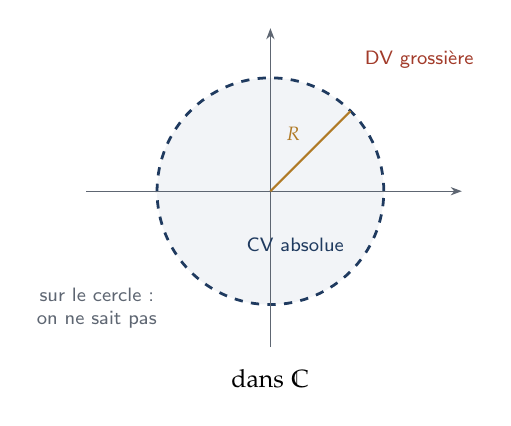
\begin{tikzpicture}[scale=0.9]
\fill[Fond] (0,0) circle (1.6);
\draw[Bleu,line width=1pt,dashed] (0,0) circle (1.6);
\draw[Gris,-{Stealth[length=4pt]}] (-2.6,0)--(2.7,0); \draw[Gris,-{Stealth[length=4pt]}] (0,-2.2)--(0,2.3);
\draw[Ocre,line width=0.8pt] (0,0)--(1.13,1.13) node[midway,above left,font=\scriptsize,Ocre]{$R$};
\node[font=\scriptsize\sffamily,Bleu] at (0.35,-0.75) {CV absolue};
\node[font=\scriptsize\sffamily,Brique] at (2.1,1.85) {DV grossière};
\node[font=\scriptsize\sffamily,Gris,align=center] at (-2.45,-1.65) {sur le cercle :\\on ne sait pas};
\node[font=\small] at (0,-2.65) {dans $\C$};
\end{tikzpicture}\hspace{1.5cm}
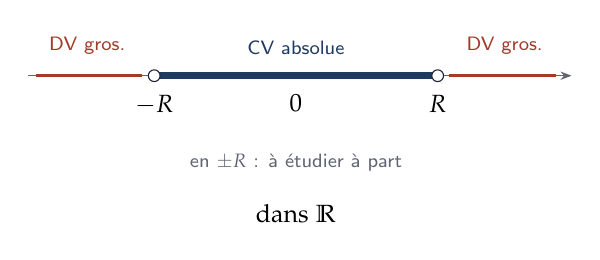
\begin{tikzpicture}
\draw[Gris,-{Stealth[length=4pt]}] (-3.4,0)--(3.5,0);
\draw[Bleu,line width=2.4pt] (-1.8,0)--(1.8,0);
\draw[Brique,line width=1pt] (-3.3,0)--(-1.95,0); \draw[Brique,line width=1pt] (1.95,0)--(3.3,0);
\node[circle,draw=Ink,fill=white,inner sep=1.5pt] at (-1.8,0) {}; \node[circle,draw=Ink,fill=white,inner sep=1.5pt] at (1.8,0) {};
\node[below,font=\small] at (-1.8,-0.12) {$-R$}; \node[below,font=\small] at (1.8,-0.12) {$R$}; \node[below,font=\small] at (0,-0.12) {$0$};
\node[above,font=\scriptsize\sffamily,Bleu] at (0,0.15) {CV absolue};
\node[above,font=\scriptsize\sffamily,Brique] at (-2.65,0.15) {DV gros.}; \node[above,font=\scriptsize\sffamily,Brique] at (2.65,0.15) {DV gros.};
\node[font=\scriptsize\sffamily,Gris] at (0,-1.1) {en $\pm R$ : à étudier à part};
\node[font=\small] at (0,-1.75) {dans $\R$};
\end{tikzpicture}
\caption{Le rayon de convergence : convergence absolue strictement à l'intérieur, divergence grossière strictement à l'extérieur.}
\label{f:disque}
\end{figure}

\begin{definition}
Si $R>0$, l'intervalle $]-R,R[$ (cas réel) est l'\emph{intervalle ouvert de convergence} ; le disque $\{z\in\C:|z|<R\}$ (cas
complexe) est le \emph{disque ouvert de convergence}.
\end{definition}

\begin{exemple}[le bord peut tout faire]
Les trois séries $\sum z^n$, $\sum\frac{z^n}n$, $\sum\frac{z^n}{n^2}$ ont le même rayon $R=1$ (§\ref{ss:calcul}). En $z=1$ : la
première diverge (grossièrement), la deuxième diverge (série harmonique), la troisième converge. En $z=-1$ : la première diverge,
la deuxième converge (série alternée), la troisième converge.
\end{exemple}

\begin{proposition}[encadrer le rayon]\label{p:encadre}
Soit $z_0\in\C$.
\begin{enumerate}
\item Si $\sum a_nz_0^n$ converge (ou si $(a_nz_0^n)$ est bornée), alors $R\geq|z_0|$.
\item Si $\sum a_nz_0^n$ diverge, alors $R\leq|z_0|$.
\item Si $\sum a_nz_0^n$ converge sans converger absolument, alors $R=|z_0|$.
\end{enumerate}
\end{proposition}

\begin{proof}
Ce sont les contraposées du théorème~\ref{t:rayon} : $|z_0|>R$ entraîne la divergence, $|z_0|<R$ la convergence absolue. Dans le
cas 3, on n'a ni $|z_0|<R$ ni $|z_0|>R$.
\end{proof}

\begin{exemple}
$\sum\frac{(-1)^n}n$ converge sans converger absolument : la série entière $\sum\frac{z^n}n$ a pour rayon $R=|-1|=1$.
\end{exemple}

\serie{Exercices}

\begin{exo}{se-encadre}{1}{encadrer un rayon}
Une série entière $\sum a_nz^n$ converge pour $z=\sqrt2\,i$ et diverge pour $z=1+i$. Quel est son rayon de convergence ?
\end{exo}

\begin{exo}{se-bord}{2}{rayon et comportement au bord}
Déterminer le rayon de convergence de $\sum\frac{x^n}{\sqrt n}$ ($n\geq1$) et la nature de la série pour $x=1$ et $x=-1$.
\end{exo}

% =====================================================================
\subsection{Calcul du rayon de convergence}\label{ss:calcul}

\subsubsection*{Comparaison et équivalents}

\begin{proposition}[comparaison]\label{p:comp}
Soient $\sum a_nz^n$ et $\sum b_nz^n$ de rayons $R_a$ et $R_b$. Si $|a_n|\leq|b_n|$ à partir d'un certain rang (ou plus
généralement si $a_n=O(b_n)$), alors $R_a\geq R_b$.
\end{proposition}

\begin{proof}
Si $|z|<R_b$, $\sum|b_nz^n|$ converge, donc $\sum|a_nz^n|$ aussi (comparaison de séries à termes positifs) : $|z|\leq R_a$. Tout
$|z|<R_b$ vérifie $|z|\leq R_a$, donc $R_b\leq R_a$.
\end{proof}

\begin{proposition}[équivalents]\label{p:equiv}
Si $|a_n|\sim|b_n|$, les séries entières $\sum a_nz^n$ et $\sum b_nz^n$ ont le même rayon.
\end{proposition}

\begin{proof}
Pour tout $z$, $|a_nz^n|\sim|b_nz^n|$ : les séries à termes positifs $\sum|a_nz^n|$ et $\sum|b_nz^n|$ ont la même nature, et le
rayon se lit sur la convergence absolue.
\end{proof}

\begin{exemple}
$\sum\sin(n)\,z^n$ : $|\sin n|\leq1$ donc $R\geq1$ (comparaison avec $\sum z^n$) ; en $z=1$, $\sin n\not\to0$ et la série diverge,
donc $R\leq1$. Ainsi $R=1$.\\
$\sum\left(\frac\pi2-\arctan n\right)z^n$ : $\frac\pi2-\arctan n=\arctan\frac1n\sim\frac1n$, même rayon que $\sum\frac{z^n}n$ : $R=1$.
\end{exemple}

\subsubsection*{Règle de d'Alembert}

\begin{methode}{Rayon par la règle de d'Alembert}\label{m:dalembert}
On applique la règle de d'Alembert à la \emph{série numérique} $\sum|a_nz^n|$, pour $z\neq0$ fixé :
\begin{enumerate}
\item calculer $\dfrac{|a_{n+1}z^{n+1}|}{|a_nz^n|}=\dfrac{|a_{n+1}|}{|a_n|}\,|z|$ et sa limite $\ell(z)$ ;
\item si $\ell(z)<1$ : convergence absolue, donc $R\geq|z|$ ; si $\ell(z)>1$ : divergence grossière, donc $R\leq|z|$ ;
\item conclure : si $\frac{|a_{n+1}|}{|a_n|}\to L$, alors $R=\frac1L$ (avec $\frac10=+\infty$ et $\frac1{+\infty}=0$).
\end{enumerate}
\end{methode}

\begin{exemple}
$\sum\frac{z^n}{n!}$ : $\frac{|z|}{n+1}\to0<1$ pour tout $z$, donc $R=+\infty$. \quad
$\sum n^nz^n$ : $\frac{(n+1)^{n+1}}{n^n}|z|=(n+1)\left(1+\frac1n\right)^n|z|\to+\infty$ pour $z\neq0$, donc $R=0$.
\end{exemple}

\begin{attention}
Si une infinité de coefficients sont nuls (série « lacunaire », comme $\sum\frac{x^{2n}}n$), le quotient $\frac{a_{n+1}}{a_n}$ n'a pas
de sens. On applique alors d'Alembert au terme \emph{effectivement présent} : $\left|\frac{x^{2n+2}/(n+1)}{x^{2n}/n}\right|=\frac n{n+1}x^2\to x^2$.
Convergence absolue si $x^2<1$, divergence si $x^2>1$ : $R=1$.
\end{attention}

\begin{proposition}\label{p:nalpha}
Pour tout $\alpha\in\R$, la série $\sum n^\alpha z^n$ a pour rayon $1$. Plus généralement, $\sum a_nz^n$ et $\sum n^\alpha a_nz^n$
ont le même rayon ; en particulier $\sum a_nz^n$ et $\sum na_nz^n$ ont le même rayon.
\end{proposition}

\begin{proof}
D'Alembert : $\left(\frac{n+1}n\right)^\alpha|z|\to|z|$, donc $R=1$. Pour le cas général, soit $R$ le rayon de $\sum a_nz^n$ et $R'$
celui de $\sum n^\alpha a_nz^n$. Si $|z|<R$, on choisit $r$ avec $|z|<r<R$ : $|n^\alpha a_nz^n|=|a_nr^n|\cdot n^\alpha\left(\frac{|z|}r\right)^n$,
produit d'une suite bornée et d'une suite qui tend vers $0$ (croissances comparées) ; donc $(n^\alpha a_nz^n)$ est bornée et
$R'\geq|z|$. Ainsi $R'\geq R$ ; en échangeant les rôles (avec $-\alpha$), $R\geq R'$.
\end{proof}

\subsubsection*{Somme et produit de Cauchy}

\begin{proposition}[somme]\label{p:somme}
Soient $\sum a_nz^n$ et $\sum b_nz^n$ de rayons $R_a$, $R_b$, et $R$ le rayon de $\sum(a_n+b_n)z^n$. Alors $R\geq\min(R_a,R_b)$,
avec égalité si $R_a\neq R_b$ ; pour $|z|<\min(R_a,R_b)$, $\sum_{n=0}^{+\infty}(a_n+b_n)z^n=\sum_{n=0}^{+\infty}a_nz^n+\sum_{n=0}^{+\infty}b_nz^n$.
Pour $\lambda\neq0$, $\sum\lambda a_nz^n$ a pour rayon $R_a$.
\end{proposition}

\begin{proof}
Si $|z|<\min(R_a,R_b)$, les deux séries convergent, donc leur somme. Si $R_a<R_b$ et $R_a<|z|<R_b$, $\sum a_nz^n$ diverge et
$\sum b_nz^n$ converge : la somme diverge, donc $R\leq R_a$.
\end{proof}

\begin{theoreme}[produit de Cauchy]\label{t:cauchy}
Soient $\sum a_nz^n$ et $\sum b_nz^n$ de rayons $R_a$, $R_b$, et $c_n=\sum_{k=0}^na_kb_{n-k}$. La série entière $\sum c_nz^n$ a
un rayon $R\geq\min(R_a,R_b)$ et, pour $|z|<\min(R_a,R_b)$ :
\[\sum_{n=0}^{+\infty}c_nz^n=\left(\sum_{n=0}^{+\infty}a_nz^n\right)\left(\sum_{n=0}^{+\infty}b_nz^n\right).\]
\end{theoreme}

\begin{proof}
Pour $|z|<\min(R_a,R_b)$, les deux séries convergent absolument ; leur produit de Cauchy (chapitre 7) converge absolument, de
somme le produit des sommes, et son terme général est $\sum_{k=0}^na_kz^kb_{n-k}z^{n-k}=c_nz^n$.
\end{proof}

\begin{exemple}
Avec $a_n=b_n=1$ : $c_n=n+1$ et, pour $|z|<1$, $\displaystyle\sum_{n=0}^{+\infty}(n+1)z^n=\frac1{(1-z)^2}$.
\end{exemple}

\begin{methode}{Déterminer un rayon de convergence}\label{m:rayon}
\begin{enumerate}
\item Coefficients avec factorielles, puissances $n$-ièmes : d'Alembert (méthode~\ref{m:dalembert}).
\item Coefficients avec un équivalent simple ($\frac{C}{n^\alpha}$, $C\lambda^n$) : proposition~\ref{p:equiv}, puis $R=1$ ou $R=\frac1{|\lambda|}$.
\item Coefficients bornés, oscillants ($\cos n$, $\sin n$, $e^{in}$) : comparaison pour $R\geq1$, puis un point où la série diverge
pour $R\leq1$.
\item Série lacunaire ($z^{2n}$, $z^{3n}$\dots) : d'Alembert sur le terme présent, ou changement de variable $Z=z^2$.
\item Toujours possible : revenir à la définition (bornitude de $a_nr^n$) ou à la proposition~\ref{p:encadre}.
\end{enumerate}
\end{methode}

\serie{Exercices}

\begin{exo}{se-rayons}{2}{rayons de convergence}
Déterminer le rayon de convergence des séries entières :
\begin{gather*}\text{(a)}\ \sum e^{\cos n}z^n\qquad\text{(b)}\ \sum\frac{e^{in}}{1+in}z^n\qquad\text{(c)}\ \sum_{n\geq2}\frac{(-1)^n}{n(n-1)}z^n\\
\text{(d)}\ \sum\frac{(2n)!}{(n!)^2}z^n\qquad\text{(e)}\ \sum2^nz^{3n}.\end{gather*}
\end{exo}

\begin{exo}{se-cauchy}{3}{un produit de Cauchy}
Soit $(a_n)$ une suite de réels non nuls telle que $\frac{a_{n+1}}{a_n}\to1$, et $S_n=\sum_{k=0}^na_k$. Justifier que
$f(x)=\sum_{n=0}^{+\infty}a_nx^n$ et $g(x)=\sum_{n=0}^{+\infty}S_nx^n$ sont définies sur $]-1,1[$, et montrer que $g(x)=\frac{f(x)}{1-x}$.
\end{exo}

% =====================================================================
\subsection{Fonction somme d'une série entière réelle}\label{ss:somme}

Dans ce paragraphe, $\sum a_nx^n$ est une série entière d'une variable \emph{réelle}, de rayon $R>0$.

\begin{definition}
La \emph{fonction somme} de $\sum a_nx^n$ est $f:x\mapsto\sum_{n=0}^{+\infty}a_nx^n$. Elle est définie au moins sur $]-R,R[$, et
éventuellement en $R$ ou en $-R$ si la série y converge.
\end{definition}

\begin{exemple}
$f(x)=\sum_{n=1}^{+\infty}\frac{x^n}n$ : $R=1$ ; la série diverge en $1$ et converge en $-1$ : $f$ est définie sur $[-1,1[$.
\end{exemple}

\begin{theoreme}[continuité]\label{t:continuite}
La fonction somme est continue sur l'intervalle ouvert de convergence $]-R,R[$.
\end{theoreme}

\begin{proposition}[continuité au bord, admise]\label{p:abelradial}
Si la série converge en $x=R$, la fonction somme est continue en $R$ (à gauche) : $\displaystyle\sum_{n=0}^{+\infty}a_nR^n=\lim_{x\to R^-}f(x)$.
De même en $-R$. Autrement dit, $f$ est continue sur son ensemble de définition.
\end{proposition}

\begin{remarque}
Ce résultat (théorème d'Abel radial) est utilisé dans le cours de la classe ; sa démonstration n'est pas exigible. Il sert à
calculer des sommes de séries numériques : on calcule $f(x)$ pour $|x|<R$, puis on fait tendre $x$ vers le bord
(exemple~\ref{x:ln2}).
\end{remarque}

\begin{theoreme}[dérivation terme à terme]\label{t:derivation}
La fonction somme $f$ est dérivable sur $]-R,R[$ et
\[\forall x\in\,]-R,R[,\qquad f'(x)=\sum_{n=1}^{+\infty}na_nx^{n-1}=\sum_{n=0}^{+\infty}(n+1)a_{n+1}x^n.\]
La série dérivée $\sum na_nx^{n-1}$ a le même rayon $R$ (proposition~\ref{p:nalpha}).
\end{theoreme}

\begin{corollaire}[classe $\mathcal C^\infty$, coefficients]\label{c:cinfini}
$f$ est de classe $\mathcal C^\infty$ sur $]-R,R[$ ; pour tout $p\in\N$,
\[f^{(p)}(x)=\sum_{n=p}^{+\infty}n(n-1)\cdots(n-p+1)\,a_nx^{n-p},\qquad\text{et en particulier}\qquad a_p=\frac{f^{(p)}(0)}{p!}.\]
\end{corollaire}

\begin{proof}
On applique le théorème~\ref{t:derivation} à $f$, puis à $f'$ (qui est encore la somme d'une série entière de rayon $R$), et ainsi
de suite. En $x=0$, seul le terme $n=p$ subsiste : $f^{(p)}(0)=p!\,a_p$.
\end{proof}

\begin{theoreme}[intégration terme à terme]\label{t:integration}
La série $\sum\frac{a_n}{n+1}x^{n+1}$ a le même rayon $R$ et, si $F$ est une primitive de $f$ sur $]-R,R[$ :
\[\forall x\in\,]-R,R[,\qquad F(x)=F(0)+\sum_{n=0}^{+\infty}\frac{a_n}{n+1}x^{n+1},\]
c'est-à-dire $\displaystyle\int_0^x\sum_{n=0}^{+\infty}a_nt^n\,dt=\sum_{n=0}^{+\infty}\int_0^xa_nt^n\,dt$ : on peut intégrer terme à terme sur $[0,x]$.
\end{theoreme}

\begin{proof}
La série $\sum\frac{a_n}{n+1}x^{n+1}$ a le même rayon que $\sum a_nx^n$ (proposition~\ref{p:nalpha}, avec un décalage d'indice). Sa
somme $G$ est dérivable de dérivée $f$ (théorème~\ref{t:derivation}) et $G(0)=0$ : $G=F-F(0)$.
\end{proof}

\begin{attention}
Dériver ou intégrer terme à terme ne change \emph{pas} le rayon, mais peut changer le comportement au bord : $\sum\frac{x^n}{n^2}$
converge en $1$, sa dérivée $\sum\frac{x^{n-1}}n$ diverge en $1$. Les théorèmes s'appliquent sur l'intervalle \emph{ouvert}.
\end{attention}

\begin{exemple}[sommes à partir de la série géométrique]\label{x:ln2}
Pour $x\in\,]-1,1[$, $\frac1{1-x}=\sum_{n=0}^{+\infty}x^n$.
\begin{itemize}
\item En dérivant : $\frac1{(1-x)^2}=\sum_{n=1}^{+\infty}nx^{n-1}$, donc $\sum_{n=1}^{+\infty}nx^n=\frac x{(1-x)^2}$.
\item En intégrant sur $[0,x]$ : $-\ln(1-x)=\sum_{n=0}^{+\infty}\frac{x^{n+1}}{n+1}=\sum_{n=1}^{+\infty}\frac{x^n}n$.
\item Au bord : la série $\sum\frac{(-1)^n}n$ converge (critère des séries alternées). Par la proposition~\ref{p:abelradial},
$\sum_{n=1}^{+\infty}\frac{(-1)^n}n=\lim_{x\to-1}\big(-\ln(1-x)\big)=-\ln2$.
\end{itemize}
\end{exemple}

\begin{methode}{Calculer la somme d'une série entière}\label{m:somme}
\begin{enumerate}
\item Déterminer le rayon $R$ ; on calcule la somme sur $]-R,R[$, puis éventuellement au bord.
\item Coefficient polynomial en $n$ et terme $x^n$ (sans factorielle) : partir de $\sum x^n=\frac1{1-x}$ et \emph{dériver} ; écrire
$P(n)$ sur la base $(n+1)(n+2)$, $(n+1)$, $1$ (ou $n(n-1)$, $n$, $1$).
\item Coefficient $\frac1{n+1}$, $\frac1{n+2}$\dots : \emph{intégrer} ; fraction rationnelle en $n$ : décomposer en éléments simples.
\item Coefficient avec $n!$ : se ramener à la famille exponentielle (méthode~\ref{m:sommeexp}).
\item Contrôler en $x=0$ et sur le premier terme du développement.
\end{enumerate}
\end{methode}

\begin{exemple}
Pour $x\in\,]-1,1[$ : $n^2=(n+1)(n+2)-3(n+1)+1$, donc
$\displaystyle\sum_{n=0}^{+\infty}n^2x^n=\frac2{(1-x)^3}-\frac3{(1-x)^2}+\frac1{1-x}=\frac{x(1+x)}{(1-x)^3}$, en utilisant
$\sum(n+1)(n+2)x^n=\left(\frac1{1-x}\right)''=\frac2{(1-x)^3}$.
\end{exemple}

\serie{Exercices}

\begin{exo}{se-sommes}{2}{calculs de sommes}
Déterminer le rayon et la somme de :
\[\text{(a)}\ \sum_{n\geq0}(n+1)(-1)^nx^n\qquad\text{(b)}\ \sum_{n\geq1}\frac{x^n}{n(n+1)}\qquad\text{(c)}\ \sum_{n\geq0}\frac{x^{2n+1}}{2n+1}.\]
En déduire $\sum_{n=1}^{+\infty}\frac1{n(n+1)2^n}$.
\end{exo}

\begin{exo}{se-coef}{2}{coefficients et dérivées}
Soit $f(x)=\sum_{n=0}^{+\infty}a_nx^n$ de rayon $R>0$. Exprimer $f''(0)$, $f^{(5)}(0)$ à l'aide des $a_n$. Si $f(x)=\frac1{1-x^2}$ sur $]-1,1[$,
que valent $f^{(10)}(0)$ et $f^{(11)}(0)$ ?
\end{exo}

% =====================================================================
\subsection{Fonctions développables en série entière}\label{ss:dse}

\begin{definition}
Soit $r>0$. Une fonction $f$ est \emph{développable en série entière} (DSE) sur $]-r,r[$ s'il existe une série entière
$\sum a_nx^n$ de rayon $R\geq r$ telle que
\[\forall x\in\,]-r,r[,\qquad f(x)=\sum_{n=0}^{+\infty}a_nx^n.\]
\end{definition}

\begin{theoreme}[le DSE est la série de Taylor]\label{t:dseTaylor}
Si $f$ est DSE sur $]-r,r[$, alors $f$ est de classe $\mathcal C^\infty$ sur $]-r,r[$ et son développement est sa série de Taylor :
\[\forall x\in\,]-r,r[,\qquad f(x)=\sum_{n=0}^{+\infty}\frac{f^{(n)}(0)}{n!}x^n.\]
En particulier le développement est \emph{unique} : si $\sum a_nx^n=\sum b_nx^n$ sur $]-r,r[$, alors $a_n=b_n$ pour tout $n$.
\end{theoreme}

\begin{proof}
C'est le corollaire~\ref{c:cinfini} : $f$ est la somme d'une série entière sur $]-r,r[$, donc $\mathcal C^\infty$, et $a_n=\frac{f^{(n)}(0)}{n!}$.
Si deux séries ont la même somme, leurs coefficients sont tous égaux à $\frac{f^{(n)}(0)}{n!}$.
\end{proof}

\begin{remarque}
Si $f$ est DSE, ses développements limités en $0$ s'obtiennent en tronquant le DSE.
\end{remarque}

\subsubsection*{Quand une fonction est-elle égale à sa série de Taylor ?}

Le théorème~\ref{t:dseTaylor} ne va que dans un sens : \emph{si} $f$ est DSE, son DSE est sa série de Taylor. La réciproque est
fausse. Pour $f$ de classe $\mathcal C^\infty$, la série de Taylor existe toujours, mais deux choses peuvent mal tourner :
\begin{enumerate}
\item son rayon est nul (il existe de telles fonctions, admis) ;
\item elle converge, mais sa somme n'est pas $f$ : c'est le cas de $e^{-1/x^2}$, dont la série de Taylor est nulle
      (exercice~\ref{e:se-plat}).
\end{enumerate}
Ce qui décide, c'est le reste de la formule de Taylor.

\begin{theoreme}[caractérisation par le reste]\label{t:caracDSE}
Soit $a>0$ et $f$ de classe $\mathcal C^\infty$ sur $]-a,a[$. Alors $f$ est DSE sur $]-a,a[$ si et seulement si, pour tout
$x\in\,]-a,a[$,
\[R_n(x)=f(x)-\sum_{k=0}^n\frac{f^{(k)}(0)}{k!}x^k=\int_0^x\frac{(x-t)^n}{n!}f^{(n+1)}(t)\,dt\xrightarrow[n\to+\infty]{}0.\]
Le développement est alors la série de Taylor.
\end{theoreme}

\begin{proof}
Par la formule de Taylor (théorème~\ref{t:taylor}), $R_n(x)$ est l'écart entre $f(x)$ et la somme partielle de rang $n$ de la
série de Taylor. Donc $R_n(x)\to0$ pour tout $x\in\,]-a,a[$ si et seulement si la série de Taylor converge vers $f(x)$ sur
$]-a,a[$ ; son rayon est alors au moins $a$, et $f$ est DSE. Réciproquement, si $f$ est DSE sur $]-a,a[$, son développement
est sa série de Taylor (théorème~\ref{t:dseTaylor}), qui converge donc vers $f(x)$ : $R_n(x)\to0$.
\end{proof}

\begin{corollaire}[dérivées uniformément bornées]\label{c:bornees}
Soit $f$ de classe $\mathcal C^\infty$ sur $]-a,a[$. S'il existe $M$ tel que $|f^{(n)}(t)|\leq M$ pour tout $n\in\N$ et tout
$t\in\,]-a,a[$, alors $f$ est DSE sur $]-a,a[$.
\end{corollaire}

\begin{proof}
Par l'inégalité de Taylor-Lagrange (corollaire~\ref{c:tl}), $|R_n(x)|\leq M\frac{|x|^{n+1}}{(n+1)!}$, qui tend vers $0$ par
croissances comparées. On conclut par le théorème~\ref{t:caracDSE}.
\end{proof}

\begin{exemple}
$|\sin^{(n)}|\leq1$ et $|\cos^{(n)}|\leq1$ sur $\R$ : $\sin$ et $\cos$ sont DSE sur $\R$ (avec $M=1$). Sur $]-a,a[$,
$|\exp^{(n)}|\leq e^a$ : $\exp$ est DSE sur $]-a,a[$ pour tout $a$, donc sur $\R$. On retrouve les théorèmes~\ref{t:exp}
et~\ref{t:trigo}.
\end{exemple}

{\centering\small\renewcommand{\arraystretch}{1.3}
\begin{tabular}{@{}p{4.6cm}p{4.2cm}p{4.6cm}@{}}
\toprule
\textbf{$f$ est DSE} & \textbf{$f$ est $\mathcal C^\infty$, Taylor de rayon nul} & \textbf{$f$ est $\mathcal C^\infty$, Taylor converge vers $g\neq f$}\\\midrule
DSE $=$ série de Taylor, $R_n(x)\to0$. Ex.~: $e^x$, $\frac1{1-x}$, $\ln(1+x)$. & Existe (admis). & $R_n(x)\not\to0$. Ex.~: $e^{-1/x^2}$, Taylor nulle.\\
\bottomrule
\end{tabular}\par}

\begin{remarque}
En pratique, on étudie rarement le reste : on développe par opérations sur les DSE usuels, par dérivation ou intégration, ou par
une équation différentielle (§\ref{ss:methodes}). Le reste sert surtout à établir les DSE de base ($\exp$, $\cos$, $\sin$), ou
lorsqu'on dispose d'une majoration des dérivées.
\end{remarque}

\begin{proposition}[parité]\label{p:parite}
Si $f$ est DSE et paire, son développement ne contient que des puissances paires ; si $f$ est impaire, que des puissances impaires.
\end{proposition}

\begin{proof}
Si $f$ est paire, $\sum a_n(-x)^n=\sum a_nx^n$, donc $\sum_{n=0}^{+\infty}2a_{2p+1}x^{2p+1}=0$ sur $]-r,r[$ ; par unicité,
$a_{2p+1}=0$. Même raisonnement pour $f$ impaire.
\end{proof}

\subsubsection*{Les développements usuels}

\begin{theoreme}[géométrique, logarithme, arctangente]\label{t:usuels1}
Pour tout $x\in\,]-1,1[$ :
\begin{gather*}\frac1{1-x}=\sum_{n=0}^{+\infty}x^n,\qquad\frac1{1+x}=\sum_{n=0}^{+\infty}(-1)^nx^n,\\
\ln(1+x)=\sum_{n=1}^{+\infty}\frac{(-1)^{n+1}}nx^n,\qquad\ln(1-x)=-\sum_{n=1}^{+\infty}\frac{x^n}n,\qquad
\arctan x=\sum_{n=0}^{+\infty}\frac{(-1)^n}{2n+1}x^{2n+1}.\end{gather*}
Ces séries ont pour rayon $1$.
\end{theoreme}

\begin{proof}
Les deux premières sont des séries géométriques. Pour $\ln(1+x)$ : on intègre terme à terme $\frac1{1+t}=\sum(-1)^nt^n$ sur $[0,x]$
(théorème~\ref{t:integration}) : $\ln(1+x)=\sum_{n=0}^{+\infty}\frac{(-1)^nx^{n+1}}{n+1}$, puis on pose $k=n+1$ ; on remplace $x$ par $-x$
pour $\ln(1-x)$. Pour $\arctan$ : $\arctan'(t)=\frac1{1+t^2}=\sum_{n=0}^{+\infty}(-1)^nt^{2n}$ pour $|t|<1$, et on intègre sur $[0,x]$,
avec $\arctan0=0$.
\end{proof}

\begin{theoreme}[la série du binôme]\label{t:binome}
Pour tout $\alpha\in\R$ et tout $x\in\,]-1,1[$ :
\[(1+x)^\alpha=1+\sum_{n=1}^{+\infty}\frac{\alpha(\alpha-1)\cdots(\alpha-n+1)}{n!}x^n.\]
Si $\alpha\in\N$, la somme est finie (formule du binôme) ; sinon, le rayon vaut $1$.
\end{theoreme}

\begin{proof}
On utilise une équation différentielle (méthode~\ref{m:ed} : c'est l'exemple type). Soit $\alpha\notin\N$ et $f(x)=(1+x)^\alpha$ sur
$]-1,1[$ : $f'(x)=\alpha(1+x)^{\alpha-1}$, donc $f$ est l'unique solution du problème de Cauchy
\[(1+x)y'=\alpha y,\qquad y(0)=1\]
(théorème de Cauchy : $1+x\neq0$ sur $]-1,1[$).

\emph{Analyse.} Si $y=\sum a_nx^n$ (rayon $R>0$) est solution, alors
$(1+x)\sum_{n\geq1}na_nx^{n-1}=\sum_{n\geq0}\big((n+1)a_{n+1}+na_n\big)x^n$ doit être égal à $\sum\alpha a_nx^n$. Par unicité du DSE :
$(n+1)a_{n+1}=(\alpha-n)a_n$ pour tout $n$, et $a_0=y(0)=1$. Par récurrence, $a_n=\frac{\alpha(\alpha-1)\cdots(\alpha-n+1)}{n!}$.

\emph{Synthèse.} Ces $a_n$ sont non nuls et $\left|\frac{a_{n+1}}{a_n}\right|=\frac{|\alpha-n|}{n+1}\to1$ : le rayon est $1$ (d'Alembert). Sur $]-1,1[$,
la somme $y$ vérifie l'équation (les calculs de l'analyse sont des équivalences) et $y(0)=1$.

\emph{Conclusion.} $f$ et $y$ sont solutions du même problème de Cauchy sur $]-1,1[$ : elles sont égales.
\end{proof}

\begin{exemple}
$\alpha=-\frac12$ : $\frac1{\sqrt{1+x}}=1-\frac12x+\frac38x^2-\frac5{16}x^3+\cdots$ ; en remplaçant $x$ par $-x^2$ et en intégrant, on
obtient le DSE de $\arcsin$ (TD).
\end{exemple}

\begin{theoreme}[exponentielle complexe]\label{t:expC}
Pour tout $z\in\C$, la série $\sum\frac{z^n}{n!}$ converge absolument et $\displaystyle e^z=\sum_{n=0}^{+\infty}\frac{z^n}{n!}$, où
$e^{x+iy}=e^x(\cos y+i\sin y)$. Pour tous $z,z'\in\C$, $e^{z+z'}=e^ze^{z'}$.
\end{theoreme}

\begin{proof}
Le rayon est $+\infty$ (d'Alembert). Pour $y\in\R$, en séparant les termes pairs et impairs de $\sum\frac{(iy)^n}{n!}$ (absolument
convergente) et en utilisant le théorème~\ref{t:trigo}, $\sum_{n=0}^{+\infty}\frac{(iy)^n}{n!}=\cos y+i\sin y=e^{iy}$. Ensuite, le produit de
Cauchy de $\sum\frac{x^n}{n!}$ et $\sum\frac{(iy)^n}{n!}$ a pour terme $\sum_{k=0}^n\frac{x^k(iy)^{n-k}}{k!(n-k)!}=\frac{(x+iy)^n}{n!}$ (binôme) ;
donc $e^xe^{iy}=\sum\frac{(x+iy)^n}{n!}$. Le même calcul avec $z$ et $z'$ donne $e^{z+z'}=e^ze^{z'}$.
\end{proof}

\begin{table}[h]
\centering
\small
\renewcommand{\arraystretch}{1.55}
\begin{tabular}{@{}>{$}l<{$}>{$}l<{$}c@{}}
\toprule
\text{Fonction} & \text{Développement en série entière} & Rayon\\\midrule
e^x & \sum_{n=0}^{+\infty}\frac{x^n}{n!} & $+\infty$\\
\ch x,\quad\sh x & \sum_{n=0}^{+\infty}\frac{x^{2n}}{(2n)!},\quad\sum_{n=0}^{+\infty}\frac{x^{2n+1}}{(2n+1)!} & $+\infty$\\
\cos x,\quad\sin x & \sum_{n=0}^{+\infty}\frac{(-1)^nx^{2n}}{(2n)!},\quad\sum_{n=0}^{+\infty}\frac{(-1)^nx^{2n+1}}{(2n+1)!} & $+\infty$\\
\frac1{1-x},\quad\frac1{1+x} & \sum_{n=0}^{+\infty}x^n,\quad\sum_{n=0}^{+\infty}(-1)^nx^n & $1$\\
\ln(1+x),\quad\ln(1-x) & \sum_{n=1}^{+\infty}\frac{(-1)^{n+1}}nx^n,\quad-\sum_{n=1}^{+\infty}\frac{x^n}n & $1$\\
\arctan x & \sum_{n=0}^{+\infty}\frac{(-1)^n}{2n+1}x^{2n+1} & $1$\\
(1+x)^\alpha & 1+\sum_{n=1}^{+\infty}\frac{\alpha(\alpha-1)\cdots(\alpha-n+1)}{n!}x^n & $1$ ($\alpha\notin\N$)\\\bottomrule
\end{tabular}
\caption{Développements en série entière usuels, à connaître par cœur.}
\label{t:tableau}
\end{table}

\serie{Exercices}

\begin{exo}{se-unicite}{2}{unicité et parité}
\begin{enumerate}
\item Sans calcul, que valent les coefficients d'indice impair du DSE de $x\mapsto\frac1{1+x^2}$ ? Le vérifier sur le développement.
\item Retrouver le DSE de $\ch$ à partir de celui de $\sh$, par dérivation.
\item Montrer que la fonction $x\mapsto\frac{\sin x}x$, prolongée par $1$ en $0$, est de classe $\mathcal C^\infty$ sur $\R$.
\end{enumerate}
\end{exo}

% =====================================================================
\subsection{Développer une fonction en série entière}\label{ss:methodes}

Pour développer une fonction, on n'utilise presque jamais directement la série de Taylor (le reste est difficile à majorer) :
on se ramène aux développements usuels.

\begin{methode}{Développer par opérations sur les DSE usuels}\label{m:operations}
\begin{enumerate}
\item \emph{Substitution} : remplacer $x$ par $-x$, $ax$, $x^2$, $-x^2$ dans un DSE usuel (le domaine change : $\frac1{1+x^2}$ pour $|x|<1$).
\item \emph{Combinaison linéaire} : sur l'intersection des intervalles de convergence.
\item \emph{Produit de Cauchy} : sur l'intersection, avec $c_n=\sum_{k=0}^na_kb_{n-k}$.
\item \emph{Dérivation, intégration} : si $f'$ (ou une primitive) a un DSE connu ; ne pas oublier la constante $f(0)$.
\item \emph{Éléments simples} : une fraction rationnelle sans pôle en $0$ se décompose en $\frac a{x-\lambda}=-\frac a\lambda\cdot\frac1{1-x/\lambda}$, valable pour $|x|<|\lambda|$.
\end{enumerate}
\end{methode}

\begin{exemple}[éléments simples]
$\dfrac1{x^2-5x+6}=\dfrac1{x-3}-\dfrac1{x-2}=\dfrac12\cdot\dfrac1{1-\frac x2}-\dfrac13\cdot\dfrac1{1-\frac x3}
=\sum_{n=0}^{+\infty}\left(\frac1{2^{n+1}}-\frac1{3^{n+1}}\right)x^n$, pour $|x|<2$ (le plus petit module des pôles).
\end{exemple}

\begin{exemple}[intégration]
$\ln\dfrac{1+x}{1-x}=\ln(1+x)-\ln(1-x)=\sum_{n=1}^{+\infty}\frac{(-1)^{n+1}+1}nx^n=2\sum_{p=0}^{+\infty}\frac{x^{2p+1}}{2p+1}$ pour $|x|<1$.
\end{exemple}

\begin{methode}{Développer par une équation différentielle}\label{m:ed}
\begin{enumerate}
\item Trouver une équation différentielle linéaire (et des conditions initiales) vérifiée par $f$ : on dérive $f$ et on cherche
une relation.
\item \emph{Analyse} : on suppose $y=\sum a_nx^n$ solution ; on dérive terme à terme, on réindexe pour avoir partout $x^n$, et
l'unicité du DSE donne une relation de récurrence sur les $a_n$.
\item On résout la récurrence (avec les conditions initiales $a_0=y(0)$, $a_1=y'(0)$).
\item \emph{Synthèse} : calculer le rayon $R$ de la série obtenue ; sur $]-R,R[$, sa somme est solution.
\item \emph{Conclure} par l'unicité de la solution du problème de Cauchy, sur un intervalle où le coefficient de $y'$ (ou $y''$) ne
s'annule pas.
\end{enumerate}
\end{methode}

\begin{exemple}
$f(x)=e^{-x^2/2}$ vérifie $y'+xy=0$, $y(0)=1$. Avec $y=\sum a_nx^n$ : $\sum_{n\geq0}(n+1)a_{n+1}x^n+\sum_{n\geq1}a_{n-1}x^n=0$,
donc $a_1=0$ et $(n+1)a_{n+1}=-a_{n-1}$. Les termes impairs sont nuls et $a_{2p}=\frac{(-1)^p}{2^pp!}$ : on retrouve
$e^{-x^2/2}=\sum\frac{(-x^2/2)^p}{p!}$, ce que donnait aussi une substitution.
\end{exemple}

\begin{methode}{Chercher les solutions DSE d'une équation différentielle}\label{m:soled}
Même analyse que la méthode~\ref{m:ed} (relation de récurrence), puis : on résout la récurrence, on calcule le rayon, on reconnaît
si possible la somme (DSE usuels) et on conclut que, sur $]-R,R[$, ces fonctions sont exactement les solutions DSE.
\end{methode}

\serie{Exercices}

\begin{exo}{se-dse}{2}{développements en série entière}
Développer en série entière au voisinage de $0$, en précisant le rayon :
\[\text{(a)}\ \frac1{(1-x)(1-2x)}\qquad\text{(b)}\ \ln(1+x-2x^2)\qquad\text{(c)}\ \frac{e^x}{1-x}.\]
En (c), donner la forme générale du coefficient et les quatre premiers termes.
\end{exo}

\begin{exo}{se-ed}{3}{une équation différentielle}
Déterminer les solutions DSE de l'équation $xy''+y'-y=0$, puis celle qui vérifie $y(0)=1$. Préciser le rayon.
\end{exo}

% =====================================================================
\subsection{Quelle méthode ? Synthèse}\label{ss:synthese}

\begin{figure}[h]
\centering
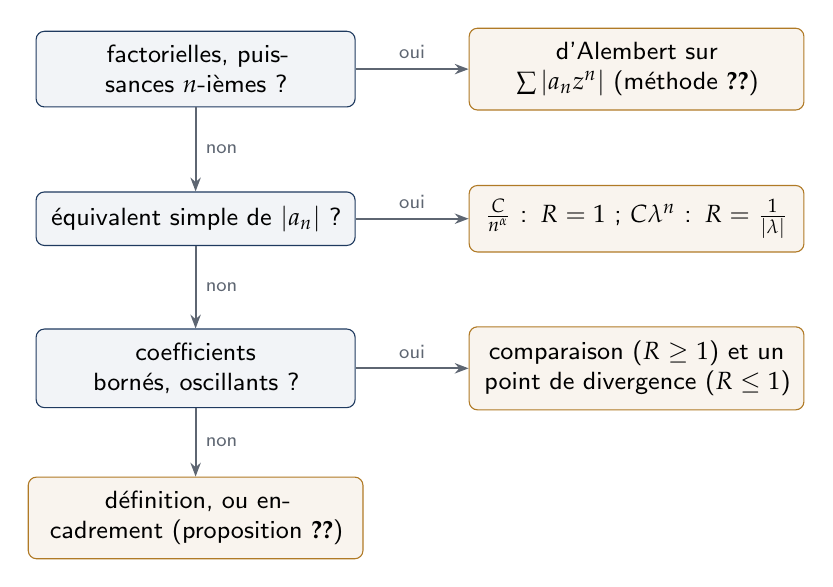
\begin{tikzpicture}[
  q/.style={draw=Bleu,fill=Fond,rounded corners=3pt,font=\small\sffamily,align=center,inner sep=5pt,text width=3.7cm},
  r/.style={draw=Ocre,fill=Ocre!8,rounded corners=3pt,font=\small\sffamily,align=center,inner sep=5pt,text width=3.9cm},
  f/.style={-{Stealth[length=5pt]},Gris,line width=0.7pt},
  l/.style={font=\scriptsize\sffamily,Gris}]
\node[q] (a) at (0,0) {factorielles, puissances $n$-ièmes ?};
\node[r] (a2) at (5.6,0) {d'Alembert sur $\sum|a_nz^n|$ (méthode~\ref{m:dalembert})};
\node[q] (b) at (0,-1.9) {équivalent simple de $|a_n|$ ?};
\node[r] (b2) at (5.6,-1.9) {$\frac C{n^\alpha}$ : $R=1$ ;\ $C\lambda^n$ : $R=\frac1{|\lambda|}$};
\node[q] (c) at (0,-3.8) {coefficients bornés, oscillants ?};
\node[r] (c2) at (5.6,-3.8) {comparaison ($R\geq1$) et un point de divergence ($R\leq1$)};
\node[r] (d) at (0,-5.7) {définition, ou encadrement (proposition~\ref{p:encadre})};
\draw[f] (a) -- node[l,above]{oui} (a2); \draw[f] (a) -- node[l,right]{non} (b);
\draw[f] (b) -- node[l,above]{oui} (b2); \draw[f] (b) -- node[l,right]{non} (c);
\draw[f] (c) -- node[l,above]{oui} (c2); \draw[f] (c) -- node[l,right]{non} (d);
\end{tikzpicture}
\caption{Déterminer un rayon de convergence : l'ordre des questions (série lacunaire : d'Alembert sur le terme présent).}
\label{f:arbre}
\end{figure}

\begin{center}
\renewcommand{\arraystretch}{1.35}
\small
\begin{tabular}{p{0.36\linewidth}p{0.57\linewidth}}
\hline
\textbf{On demande\dots} & \textbf{Outil}\\\hline
le rayon de $\sum a_nz^n$ & arbre ci-dessus ; d'Alembert sur la série numérique\\
la nature au bord ($x=\pm R$) & séries numériques : Riemann, séries alternées, divergence grossière\\
la somme, coefficient polynomial en $n$ & dériver $\frac1{1-x}$ ; base $(n+1)(n+2)$, $n+1$, $1$\\
la somme, coefficient $\frac1{n+k}$ ou fraction & intégrer ; éléments simples ; $\ln(1-x)$\\
la somme, coefficient avec $n!$ & famille exponentielle ; $x=\pm t^2$\\
une somme numérique $\sum a_n$ & reconnaître $f(1)$ ou $f(-1)$ ; continuité au bord\\
le DSE d'une fonction & substitution, opérations, dérivation, intégration, éléments simples\\
le DSE d'une fonction « compliquée » & équation différentielle (méthode~\ref{m:ed})\\
$f^{(p)}(0)$ & $p!\,a_p$ (corollaire~\ref{c:cinfini})\\\hline
\end{tabular}
\end{center}

\begin{attention}\textbf{Pièges fréquents.}
\begin{itemize}[leftmargin=1.1em]
\item Conclure au bord à partir du rayon : en $|z|=R$, tout peut arriver.
\item Appliquer d'Alembert aux coefficients $a_n$ quand une infinité d'entre eux sont nuls.
\item Écrire un DSE sans préciser l'intervalle de validité (par exemple $\frac1{1+x^2}$ n'est développé que pour $|x|<1$).
\item Oublier la constante en intégrant ($F(0)$) ou le premier terme en dérivant (l'indice de départ change).
\item Croire qu'une fonction $\mathcal C^\infty$ est toujours égale à sa série de Taylor.
\end{itemize}
\end{attention}

\begin{essentiel}
\begin{itemize}[leftmargin=1.1em,itemsep=2pt]
\item Taylor avec reste intégral : $f(x)$ est la somme de sa série de Taylor si et seulement si le reste tend vers $0$ ; si les dérivées sont uniformément bornées, $f$ est DSE. $\mathcal C^\infty$ ne suffit pas.
\item Rayon $R$ : convergence absolue pour $|z|<R$, divergence grossière pour $|z|>R$, rien de général pour $|z|=R$.
\item Calcul du rayon : d'Alembert sur $\sum|a_nz^n|$, équivalents, comparaison ; $\sum a_nz^n$ et $\sum na_nz^n$ ont le même rayon.
\item Sur $]-R,R[$, la somme est $\mathcal C^\infty$, se dérive et s'intègre terme à terme, et $a_n=\frac{f^{(n)}(0)}{n!}$.
\item DSE usuels (tableau~\ref{t:tableau}) ; on développe par opérations, dérivation, intégration, ou par une équation différentielle.
\end{itemize}
\end{essentiel}

% =====================================================================
%                              CORRIGÉS
% =====================================================================
\clearpage
\renewcommand{\ongletcouleur}{Ocre}
\section{Corrigés}\label{sec:corriges-se}

\begin{corrige}{se-fexp}
\q{(a)} Si $x=t^2>0$ ($t=\sqrt x$) : $\sum_{n=0}^{+\infty}\frac{(-1)^nt^{2n}}{(2n+1)!}=\frac1t\sum_{n=0}^{+\infty}\frac{(-1)^nt^{2n+1}}{(2n+1)!}=\frac{\sin t}t=\frac{\sin\sqrt x}{\sqrt x}$.
Si $x=-t^2<0$ : $(-1)^nx^n=t^{2n}$ et la somme vaut $\frac{\sh t}t=\frac{\sh\sqrt{-x}}{\sqrt{-x}}$. Si $x=0$ : la somme vaut $1$.
\q{(b)} $\frac{n+1}{n!}=\frac n{n!}+\frac1{n!}$ et $\sum_{n\geq1}\frac{x^n}{(n-1)!}=x\sum_{k\geq0}\frac{x^k}{k!}=xe^x$. Donc la somme vaut $(x+1)e^x$.
\q{(c)} $\frac{e^x+e^{-x}}2=\ch x$ garde les termes d'indice pair, $\cos x$ les garde avec le signe $(-1)^p$ ; dans $\frac{\ch x+\cos x}2$,
les termes $\frac{x^{2p}}{(2p)!}$ ont pour coefficient $\frac{1+(-1)^p}2$, qui vaut $1$ si $p$ est pair et $0$ sinon. Donc
$\sum_{n=0}^{+\infty}\frac{x^{4n}}{(4n)!}=\frac{\ch x+\cos x}2$.
\gain{pour isoler une classe d'indices modulo $2$ ou $4$, on combine $f(x)$ et $f(-x)$, ou $e^x,e^{-x},e^{ix},e^{-ix}$.}
\end{corrige}

\begin{corrige}{se-plat}
\q{1.} Pour $n=0$, $P_0=1$. Si $f^{(n)}(x)=\frac{P_n(x)}{x^{3n}}e^{-1/x^2}$, on dérive (avec $\left(e^{-1/x^2}\right)'=\frac2{x^3}e^{-1/x^2}$) :
\begin{align*}f^{(n+1)}(x)&=\left(\frac{P_n'(x)x^{3n}-3nx^{3n-1}P_n(x)}{x^{6n}}+\frac{2P_n(x)}{x^{3n+3}}\right)e^{-1/x^2}\\
&=\frac{x^3P_n'(x)-3nx^2P_n(x)+2P_n(x)}{x^{3n+3}}e^{-1/x^2},\end{align*}
et $P_{n+1}=X^3P_n'-3nX^2P_n+2P_n$ est un polynôme.
\q{2.} Pour tout $k\in\N$, $\frac1{x^k}e^{-1/x^2}\to0$ quand $x\to0$ (on pose $X=\frac1{x^2}$ : $X^{k/2}e^{-X}\to0$, croissances comparées).
Donc $f^{(n)}(x)\to0$ en $0$. Par récurrence, $f^{(n)}$ est continue en $0$ avec $f^{(n)}(0)=0$, et dérivable en $0$ :
$\frac{f^{(n)}(x)-0}{x}=\frac{P_n(x)}{x^{3n+1}}e^{-1/x^2}\to0$. Ainsi $f$ est $\mathcal C^\infty$ et toutes ses dérivées en $0$ sont nulles.
\q{3.} La série de Taylor est $\sum0\cdot x^n$, de somme nulle. Or $f(x)>0$ pour $x\neq0$ : $f$ n'est égale à sa série de Taylor sur
aucun intervalle $]-r,r[$, donc $f$ n'est pas DSE (théorème~\ref{t:dseTaylor}).
\end{corrige}

\begin{corrige}{se-encadre}
La série converge en $\sqrt2\,i$, donc $R\geq|\sqrt2\,i|=\sqrt2$ ; elle diverge en $1+i$, donc $R\leq|1+i|=\sqrt2$. Ainsi $R=\sqrt2$.
\end{corrige}

\begin{corrige}{se-bord}
D'Alembert : $\sqrt{\frac n{n+1}}\,|x|\to|x|$, donc $R=1$. En $x=1$ : $\sum\frac1{\sqrt n}$ diverge (Riemann, $\frac12\leq1$). En $x=-1$ :
$\sum\frac{(-1)^n}{\sqrt n}$ converge (critère des séries alternées : $\frac1{\sqrt n}$ décroît vers $0$), sans converger absolument ; on
retrouve $R=1$ par la proposition~\ref{p:encadre}.
\end{corrige}

\begin{corrige}{se-rayons}
\q{(a)} $e^{-1}\leq e^{\cos n}\leq e$ : par comparaison avec $\sum e^{-1}z^n$ et $\sum ez^n$ (rayon $1$), $1\leq R\leq1$. Donc $R=1$.
\q{(b)} $\left|\frac{e^{in}}{1+in}\right|=\frac1{\sqrt{1+n^2}}\sim\frac1n$ : même rayon que $\sum\frac{z^n}n$, $R=1$.
\q{(c)} $\left|\frac{(-1)^n}{n(n-1)}\right|\sim\frac1{n^2}$ : même rayon que $\sum\frac{z^n}{n^2}$, c'est-à-dire $1$ (proposition~\ref{p:nalpha}).
\q{(d)} $\frac{a_{n+1}}{a_n}=\frac{(2n+2)(2n+1)}{(n+1)^2}=\frac{2(2n+1)}{n+1}\to4$ : $R=\frac14$.
\q{(e)} Série lacunaire : pour $z\neq0$, $\frac{|2^{n+1}z^{3n+3}|}{|2^nz^{3n}|}=2|z|^3$. Convergence absolue si $2|z|^3<1$, divergence si
$2|z|^3>1$ : $R=2^{-1/3}$.
\end{corrige}

\begin{corrige}{se-cauchy}
D'Alembert : $\left|\frac{a_{n+1}x^{n+1}}{a_nx^n}\right|\to|x|$, donc $\sum a_nx^n$ a pour rayon $1$ : $f$ est définie sur $]-1,1[$. Le produit
de Cauchy de $\sum a_nx^n$ et $\sum x^n$ (rayons $1$) a pour coefficient $c_n=\sum_{k=0}^na_k\cdot1=S_n$ : son rayon est au moins $1$,
donc $g$ est définie sur $]-1,1[$, et $g(x)=f(x)\cdot\frac1{1-x}$ (théorème~\ref{t:cauchy}).
\end{corrige}

\begin{corrige}{se-sommes}
\q{(a)} $R=1$ (d'Alembert). En dérivant $\frac1{1+x}=\sum(-1)^nx^n$ : $-\frac1{(1+x)^2}=\sum_{n\geq1}(-1)^nnx^{n-1}=-\sum_{n\geq0}(-1)^n(n+1)x^n$.
Donc $\sum_{n=0}^{+\infty}(n+1)(-1)^nx^n=\frac1{(1+x)^2}$.
\q{(b)} $R=1$. $\frac1{n(n+1)}=\frac1n-\frac1{n+1}$. Pour $0<|x|<1$ : $\sum_{n\geq1}\frac{x^n}n=-\ln(1-x)$ et
$\sum_{n\geq1}\frac{x^n}{n+1}=\frac1x\sum_{k\geq2}\frac{x^k}k=\frac{-\ln(1-x)-x}x$. Donc
\[S(x)=-\ln(1-x)+\frac{\ln(1-x)+x}x=1+\frac{(1-x)\ln(1-x)}x,\qquad S(0)=0.\]
\q{(c)} $R=1$. Sa dérivée est $\sum x^{2n}=\frac1{1-x^2}=\frac12\left(\frac1{1-x}+\frac1{1+x}\right)$ ; en intégrant (valeur $0$ en $0$) :
$\sum_{n=0}^{+\infty}\frac{x^{2n+1}}{2n+1}=\frac12\ln\frac{1+x}{1-x}$.
\q{Application.} Avec $x=\frac12$ dans (b) : $\sum_{n=1}^{+\infty}\frac1{n(n+1)2^n}=1+\frac{\frac12\ln\frac12}{\frac12}=1-\ln2\approx0{,}307$.
\end{corrige}

\begin{corrige}{se-coef}
$a_p=\frac{f^{(p)}(0)}{p!}$ : $f''(0)=2a_2$, $f^{(5)}(0)=120\,a_5$. Pour $f(x)=\frac1{1-x^2}=\sum_{n=0}^{+\infty}x^{2n}$ : $a_{10}=1$ et $a_{11}=0$,
donc $f^{(10)}(0)=10!=3\,628\,800$ et $f^{(11)}(0)=0$ (fonction paire).
\end{corrige}

\begin{corrige}{se-unicite}
\q{1.} La fonction est paire : ses coefficients impairs sont nuls (proposition~\ref{p:parite}). En effet
$\frac1{1+x^2}=\sum_{n=0}^{+\infty}(-1)^nx^{2n}$ pour $|x|<1$.
\q{2.} $\sh x=\sum_{n=0}^{+\infty}\frac{x^{2n+1}}{(2n+1)!}$ (rayon $+\infty$) ; en dérivant terme à terme,
$\ch x=\sh'(x)=\sum_{n=0}^{+\infty}\frac{(2n+1)x^{2n}}{(2n+1)!}=\sum_{n=0}^{+\infty}\frac{x^{2n}}{(2n)!}$.
\q{3.} Pour $x\neq0$, $\frac{\sin x}x=\sum_{n=0}^{+\infty}\frac{(-1)^nx^{2n}}{(2n+1)!}$, et cette somme vaut $1$ en $0$. La fonction prolongée
est donc la somme d'une série entière de rayon $+\infty$ : elle est $\mathcal C^\infty$ sur $\R$ (corollaire~\ref{c:cinfini}).
\end{corrige}

\begin{corrige}{se-dse}
\q{(a)} $\frac1{(1-x)(1-2x)}=\frac2{1-2x}-\frac1{1-x}=\sum_{n=0}^{+\infty}\left(2^{n+1}-1\right)x^n$, pour $|x|<\frac12$ ; le rayon est $\frac12$
(coefficient $\sim2^{n+1}$).
\q{(b)} $1+x-2x^2=(1-x)(1+2x)$, positif près de $0$ : $\ln(1+x-2x^2)=\ln(1-x)+\ln(1+2x)=\sum_{n=1}^{+\infty}\frac{(-1)^{n+1}2^n-1}nx^n$,
valable pour $|x|<1$ et $|2x|<1$ ; le rayon est $\frac12$.
\q{(c)} Produit de Cauchy de $\sum\frac{x^n}{n!}$ ($R=+\infty$) et $\sum x^n$ ($R=1$) : pour $|x|<1$,
$\frac{e^x}{1-x}=\sum_{n=0}^{+\infty}\left(\sum_{k=0}^n\frac1{k!}\right)x^n=1+2x+\frac52x^2+\frac83x^3+\cdots$. Les coefficients tendent vers
$e\neq0$ : le rayon vaut exactement $1$.
\end{corrige}

\begin{corrige}{se-ed}
\choix{analyse : on injecte $y=\sum a_nx^n$, on réindexe pour avoir $x^n$ partout, puis on identifie.}
$xy''=\sum_{n\geq2}n(n-1)a_nx^{n-1}$ et $y'=\sum_{n\geq1}na_nx^{n-1}$, donc $xy''+y'=\sum_{n\geq1}n^2a_nx^{n-1}=\sum_{n\geq0}(n+1)^2a_{n+1}x^n$.
L'équation s'écrit $\sum_{n\geq0}\big((n+1)^2a_{n+1}-a_n\big)x^n=0$ ; par unicité du DSE, $a_{n+1}=\frac{a_n}{(n+1)^2}$, donc $a_n=\frac{a_0}{(n!)^2}$.

Synthèse : $\sum\frac{x^n}{(n!)^2}$ a pour rayon $+\infty$ (d'Alembert : $\frac{|x|}{(n+1)^2}\to0$), et sa somme vérifie l'équation sur $\R$.
Les solutions DSE sont les $y=a_0\sum_{n=0}^{+\infty}\frac{x^n}{(n!)^2}$, $a_0\in\R$ ; celle qui vaut $1$ en $0$ correspond à $a_0=1$.
\piege{l'équation a pour coefficient $x$ devant $y''$, qui s'annule en $0$ : le théorème de Cauchy ne s'applique pas sur un
intervalle contenant $0$. Il n'y a qu'une droite de solutions DSE, alors que l'espace des solutions sur $]0,+\infty[$ est de dimension $2$.}
\end{corrige}

\end{document}
